%%%%%%%%%%%%%%%%%%%%%%% file template.tex %%%%%%%%%%%%%%%%%%%%%%%%%
%
% This is a general template file for the LaTeX package SVJour3
% for Springer journals.          Springer Heidelberg 2010/09/16
%
% Copy it to a new file with a new name and use it as the basis
% for your article. Delete % signs as needed.
%
% This template includes a few options for different layouts and
% content for various journals. Please consult a previous issue of
% your journal as needed.
%
%%%%%%%%%%%%%%%%%%%%%%%%%%%%%%%%%%%%%%%%%%%%%%%%%%%%%%%%%%%%%%%%%%%
\RequirePackage{fix-cm}
%
\documentclass{svjour3}                     % onecolumn (standard format)
%\documentclass[smallcondensed]{svjour3}     % onecolumn (ditto)
%\documentclass[smallextended]{svjour3}       % onecolumn (second format)
%\documentclass[twocolumn]{svjour3}          % twocolumn
%
\smartqed  % flush right qed marks, e.g. at end of proof
%
\usepackage{graphicx}
%
% \usepackage{mathptmx}      % use Times fonts if available on your TeX system
%
% insert here the call for the packages your document requires
%\usepackage{latexsym}
\usepackage{amsmath}
\usepackage{amssymb}
%\usepackage{geometry}
\usepackage{subcaption}

\usepackage{siunitx}
%\usepackage{xcolor}
\usepackage{enumitem}
\setlist{nosep}
\usepackage{footnote}

%%%
% Remove these when submitting
% We can turn the standalone tikz figures into regular figure files
%%%
\usepackage{standalone}
\usepackage{tikz}
\usetikzlibrary{patterns}
\usetikzlibrary{decorations.pathreplacing}
\usetikzlibrary{calc}
\tikzset{
    right angle quadrant/.code={
        \pgfmathsetmacro\quadranta{{1,1,-1,-1}[#1-1]}     % Arrays for selecting quadrant
        \pgfmathsetmacro\quadrantb{{1,-1,-1,1}[#1-1]}},
    right angle quadrant=1, % Make sure it is set, even if not called explicitly
    right angle length/.code={\def\rightanglelength{#1}},   % Length of symbol
    right angle length=2ex, % Make sure it is set...
    right angle symbol/.style n args={3}{
        insert path={
            let \p0 = ($(#1)!(#3)!(#2)$) in     % Intersection
                let \p1 = ($(\p0)!\quadranta*\rightanglelength!(#3)$), % Point on base line
                \p2 = ($(\p0)!\quadrantb*\rightanglelength!(#2)$) in % Point on perpendicular line
                let \p3 = ($(\p1)+(\p2)-(\p0)$) in  % Corner point of symbol
            (\p1) -- (\p3) -- (\p2)
        }
    }
}

\usepackage{csquotes}
\usepackage[USenglish]{babel}
\usepackage[backend=biber]{biblatex}

\addbibresource{articleBOS.bib}
% etc.
%
% please place your own definitions here and don't use \def but
% \newcommand{}{}
\DeclareMathOperator{\sign}{sign}
%
% Insert the name of "your journal" with
 \journalname{Experiments in Fluids}
%
\begin{document}

\title{Whole-field total density measurements by Digital Image Correlation
\thanks{Grants or other notes
about the article that should go on the front page should be
placed here. }
}


%\subtitle{Do you have a subtitle?\\ If so, write it here}

%\titlerunning{Short form of title}        % if too long for running head

\author{Alexander M. van Oers \and
       Leo R.M. Maas %etc.
}

%\authorrunning{Short form of author list} % if too long for running head

\institute{Alexander M. van Oers \at
             NIOZ Royal Netherlands Institute for Sea Research and Utrecht University, P.O. Box 59, 1790 AB Texel, The Netherlands \\
             \emph{Present address:} Faculty of Military Sciences, Netherlands Defence Academy, \\
             P.O. Box 10000, 1780 CA Den Helder, The Netherlands  %  if needed
           \and
           Leo R.M. Maas \at
              Imau, Inst. for Marine and Atmospheric research Utrecht, Utrecht University, Princetonplein 5, 3584 CC, Utrecht, The Netherlands
}

\date{Received: date / Accepted: date}
% The correct dates will be entered by the editor


\maketitle

\begin{abstract}
An optical method for the quantitative measurement of the total density field of two-dimensional stratified or homogeneous transparent fluids is presented. It is based on the Synthetic Schlieren method. Application of this method is illustrated by the determination of the static background density of a two-layer fluid and of a stratified fluid. Further aspects of the technique are illustrated by considering the dynamic total density field of a wave attractor in a stratified fluid.
\keywords{First keyword \and Second keyword \and More}
% \PACS{PACS code1 \and PACS code2 \and more}
% \subclass{MSC code1 \and MSC code2 \and more}
\end{abstract}

\section{Introduction}
\label{intro}
The Background Oriented Schlieren technique (BOS) is an optical density visualization technique \cite{meier2002computerized,raffel2015background}. First described in \cite{dalziel2000whole}, where it was called Synthetic Schlieren (SS). This technique provides whole-field measurements of density gradients. One of the strengths of this technique was the simplicity of the experimental setup. Parts of the traditional, more extensive optical setups were replaced by digital image analysis. 

In a typical SS application, perturbations (waves) in a fluid contained in a tank are imaged. Two or more images are compared using Digital Image Correlation (DIC) \cite{sutton2009image}. This comparison yields the displacements between the images. These displacements are related to the changes in the gradients of the index of refraction using a ray tracing model. These gradients of the index of refraction are related to the gradients of the density by experimentally determined data (e.g. \cite{tan2015dependence}), by the Gladstone-Dale relation for gases \cite{born2013principles} or by the Lorentz-Lorenz equation for liquids \cite{lorentz1916theory}. The density field is sometimes obtained from the gradients of the density perturbations by solving a Poisson equation \cite{venkatakrishnan2004density, verso2015background}.

In this paper we present a modification to the BOS or SS technique to directly measure the density field. We take images of static situations:  (1) before filling a tank in the experimental setup with (stratified) fluids, (2) after filling the tank with a calibration fluid and (3) after filling the tank with (stratified) fluids. Then we take images of the dynamic situations: we image, as in SS, the perturbations, or waves, traveling through a fluid. We perform DIC to obtain displacements between the images. Using a ray tracing model we relate these displacements to the index of refraction. The static images give us the background density. The dynamic images give us the dynamic density field.

The challenge of this new method is to have enough accuracy in our measurements and models to ensure that our results are useful. Determining the value of the density is more sensitive to noise than determining the density gradients of perturbations in a BOS or SS application. We also want to preserve the experimental simplicity of the BOS or SS method. In Section \ref{sec:simmod} we perform a naive application of the SS technique to try to measure the index of refraction of homogeneous water. We analyze a simple ray tracing model to determine why our naive approach failed. We show that light rays, traveling from the background through the fluid to the camera, should not travel in nearly straight lines (as in BOS or SS) but should have large deflections. We should either rotate the fluid tank or rotate (and move) our camera. We should not be placing our camera right in front of the fluid tank. 

To obtain the required accuracy in determining the density field we optimize all the steps in our method.  In Section \ref{sec:formod} we derive our ray tracing model relating displacements to the index of refraction. We call this our forward model: given an index of refraction field and experimental parameters, we can compute the displacement field of our experimental setup. This ray tracing model is a 3D model that allows the camera to be placed under an angle with respect to the fluid tank. In Section \ref{sec:cal} we describe our calibration procedure. This calibration determines accurately certain parameters in our forward model.  In Section \ref{sec:DIC} we discuss DIC. We provide references to papers that discuss techniques that allow us to get the most of our DIC procedure. We also provide information about our settings for a typical DIC calculation. We discuss best practices to get the most out of our experiments. In Section \ref{sec:invmod} we discuss how to solve our inverse model: how to obtain the index of refraction from the experimentally obtained displacements and our forward model. Section \ref{sec:res} shows three applications of our new method. In Section \ref{sec:dis} we summarize the main strengths and weaknesses of our method.

\section{Simple Model}
\label{sec:simmod}
Consider the experimental set up as shown in Figure \ref{fig:schviepalira}. Light rays travel from a camera, through a water tank onto a background with a random dot pattern.  We describe the camera as a pinhole camera with an image sensor. We place the origin of a Cartesian coordinate system at the pinhole, the location where all light rays falling on the image sensor pass through. The $z$-axis is perpendicular to the experimental setup, i.e. such that a light ray traveling along the z-axis will not be refracted by the set-up. We want to determine the position where the light rays end up, $x_6$. The light ray exits the camera with a position $x_1 = 0$ and an angle $\theta_x$. %The $x$-axis points opposite to gravity.

%\begin{figure}[hpbt]
%	\includestandalone{simplesetup}
%	\caption{A schematic view of a path of a light ray (not to scale). The numbers indicate the planes through which the light ray propagates: 1, the camera lens; 2, the start of the first glass plate; 3, the end of the first glass plate; 4, the start of the second glass plate; 5, the end of the second glass plate; 6, the screen from which the light rays originate. $n_0$, $n_1$ and $n_2$ are the index of refraction of, respectively, air, material of the tank and the fluid. The lengths are: $L_c$, the distance from camera to the first glass plate; $L_g$, the width of the glass plates; $L_t$ the width of the tank; $L_s$, the distance from the second glass plate to the screen.}
%	\label{fig:schviepalira}
%\end{figure}

\begin{figure}[htbp]
	\includestandalone[width=\textwidth]{schematicsetupangle}
	\caption{A schematic view of a path of a light ray (not to scale). The light ray in the reference state is indicated by a solid line, the light ray after filling the tank with water by a dashed line. The numbers indicate the planes through which the light ray propagates: 0, the image sensor inside the camera; 1, the camera pinhole; 2, the start of the first glass plate; 3, the end of the first glass plate; 4, the start of the second glass plate; 5, the end of the second glass plate; 6, the screen from which the light rays originate.  $n_0$, $n_1$ and $n_2$ are the index of refraction of, respectively, air, material of the tank and the fluid. The lengths (in the $z$-direction) are: $L_c$, the distance from camera to the first glass plate; $L_g$, the width of the glass plates; $L_t$ the width of the tank; $L_s$, the distance from the second glass plate to the screen.}	
\label{fig:schviepalira}	
\end{figure}

Assuming the refractive index in each section of the set up is constant, we can write for the light path,
\begin{equation}
	\label{eq:simpleline}
x(z) = x_i + z \tan \theta_i, \qquad i = 1, ... , 5,
\end{equation}
where $x_i$ is the $x$-position of the light ray at the start of each section and $\theta_i$ is the angle between the direction the ray is propagating and the $z$-axis. When encountering a discontinuous change in refractive index (when passing between the sections), we invoke Snell's law
\begin{equation}
	\label{eq:snellslaw}
n_i \sin \theta_i = \mbox{ constant},
\end{equation}
where $n_i$ is the refractive index for the $i^{th}$ section. The position $x_6$ is
%\begin{align}
%\label{eq:simplex6}
%x_6 (\theta_x, n_2) & =  (L_c+L_s) \tan \theta_x + 2 L_g \tan \arcsin \frac{n_0}{n_1} \sin \theta_x + L_t \tan \arcsin \frac{n_0}{n_2} \sin \theta_x \nonumber \\
%& =  (L_c+L_s) \tan \theta_x + \frac{2 L_g n_0 \sin \theta_x}{\sqrt{n_1^2 - n_0^2 \sin^2 \theta_x}} + \frac{L_t n_0 \sin \theta_x}{\sqrt{n_2^2 - n_0^2 \sin^2 \theta_x}}.
%\end{align}
\begin{equation}
\label{eq:simplex6}
x_6 (\theta_x, n_2) =  (L_c+L_s) \tan \theta_x + \frac{2 L_g n_0 \sin \theta_x}{\sqrt{n_1^2 - n_0^2 \sin^2 \theta_x}} + \frac{L_t n_0 \sin \theta_x}{\sqrt{n_2^2 - n_0^2 \sin^2 \theta_x}}.
\end{equation}
In this simple model, the displacement $\Delta x$ is the difference in position $x_6$ between the constant reference state, $n_2 = n_0$, and the unknown state $n_2=n$, 
%\begin{align}
%\label{eq:dexcon2}
%\Delta x = x_6 (n_2 = n_0) - x_6 (n_2 = n) & = L_t \left[ \tan \theta_x - \tan \arcsin \frac{n_0}{n} \sin \theta_x\right] \nonumber \\
%& = L_t \left[ \tan \theta_x - \frac{n_0 \sin \theta_x}{\sqrt{n^2 - n_0^2 \sin^2 \theta_x}} \right] .
%\end{align}
\begin{equation}
\label{eq:dexcon2}
\Delta x = x_6 (n_2 = n_0) - x_6 (n_2 = n) = L_t \left( \tan \theta_x - \frac{n_0 \sin \theta_x}{\sqrt{n^2 - n_0^2 \sin^2 \theta_x}} \right) .
\end{equation}
Inverting this relation we obtain the unknown refractive index $n$ as a function of the displacement
\begin{equation}
\label{eq:invdexcon2}
n =\frac{n_0 \sin(\theta_x)}{\tan(\theta_x)-\frac{\Delta x}{L_t}} \sqrt{1+\left(\tan(\theta_x)-\frac{\Delta x}{L_t}\right)^2}. % \frac{n_0 \sin \theta_x}{\sin \arctan \left( \tan \theta_x - \frac{\Delta x}{L_t} \right)} = 
\end{equation}
%The angle $\theta_x$, the displacement $\Delta x$ and unknown index of refraction $n$ are functions of the coordinate $x$. % Equation (\ref{eq:invdexcon2}) holds for each point. 

Figure \ref{fig:simmod} shows the results when using (\ref{eq:invdexcon2}) to obtain the index of refraction $n$. We have two frontal images of the experimental setup; (1) Figure \ref{fig:air0simplefrontal}, without water, and (2) Figure \ref{fig:fresh0simplefrontal}, with water.  Applying DIC we obtain; Figure \ref{fig:CCsimplefrontal} the correlation coefficient, a measure of the reliability of the method; Figure \ref{fig:DXsimplefrontal} the horizontal displacements $\Delta x$; and (3) Figure \ref{fig:DYsimplefrontal} the vertical displacements $\Delta y$. Where $\Delta x = \Delta y = 0$ is the location of the $z$-axis. We calculate the angles $\theta_x$ and $\theta_y$ with respect to this $z$-axis. Using (\ref{eq:invdexcon2}) we can compute the index of refraction $n$. Figures \ref{fig:nfromdxsimplefrontal}, \ref{fig:nfromdysimplefrontal} and \ref{fig:nfrontal} show $n$ computed from, respectively, the horizontal displacements $\Delta x$, the vertical displacements $\Delta y$ and the combined displacements.

\begin{figure}[htbp]
\begin{subfigure}{.45\linewidth}
		\centering 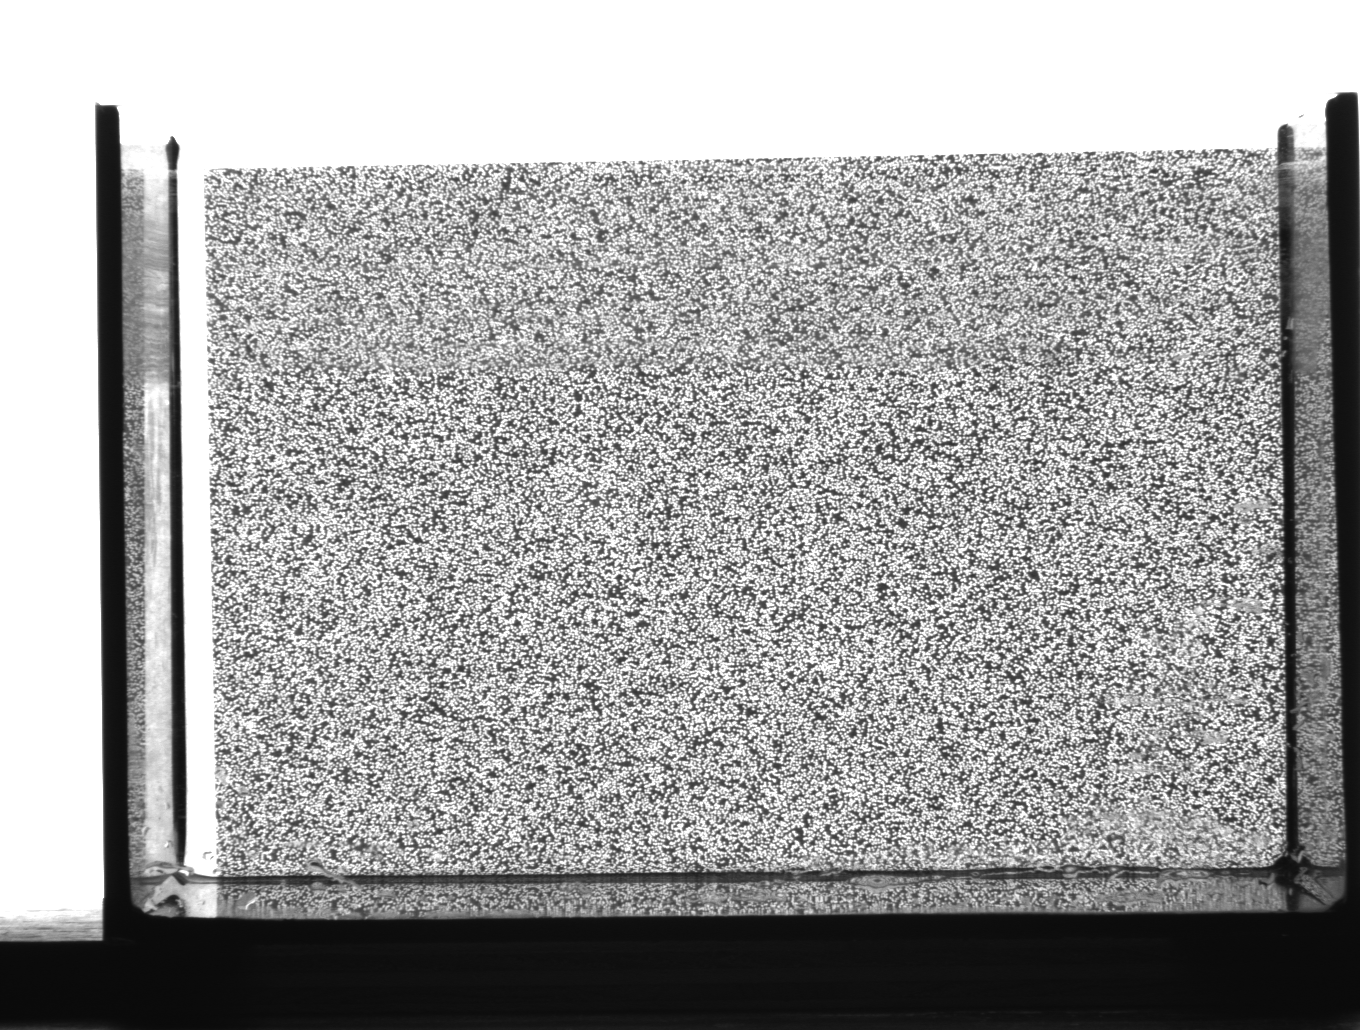
\includegraphics[width = \textwidth,keepaspectratio]{Refsimplefrontal}
		\subcaption{Reference Image: Filled with air}\label{fig:air0simplefrontal}
\end{subfigure}%
\begin{subfigure}{.45\linewidth}
	\centering 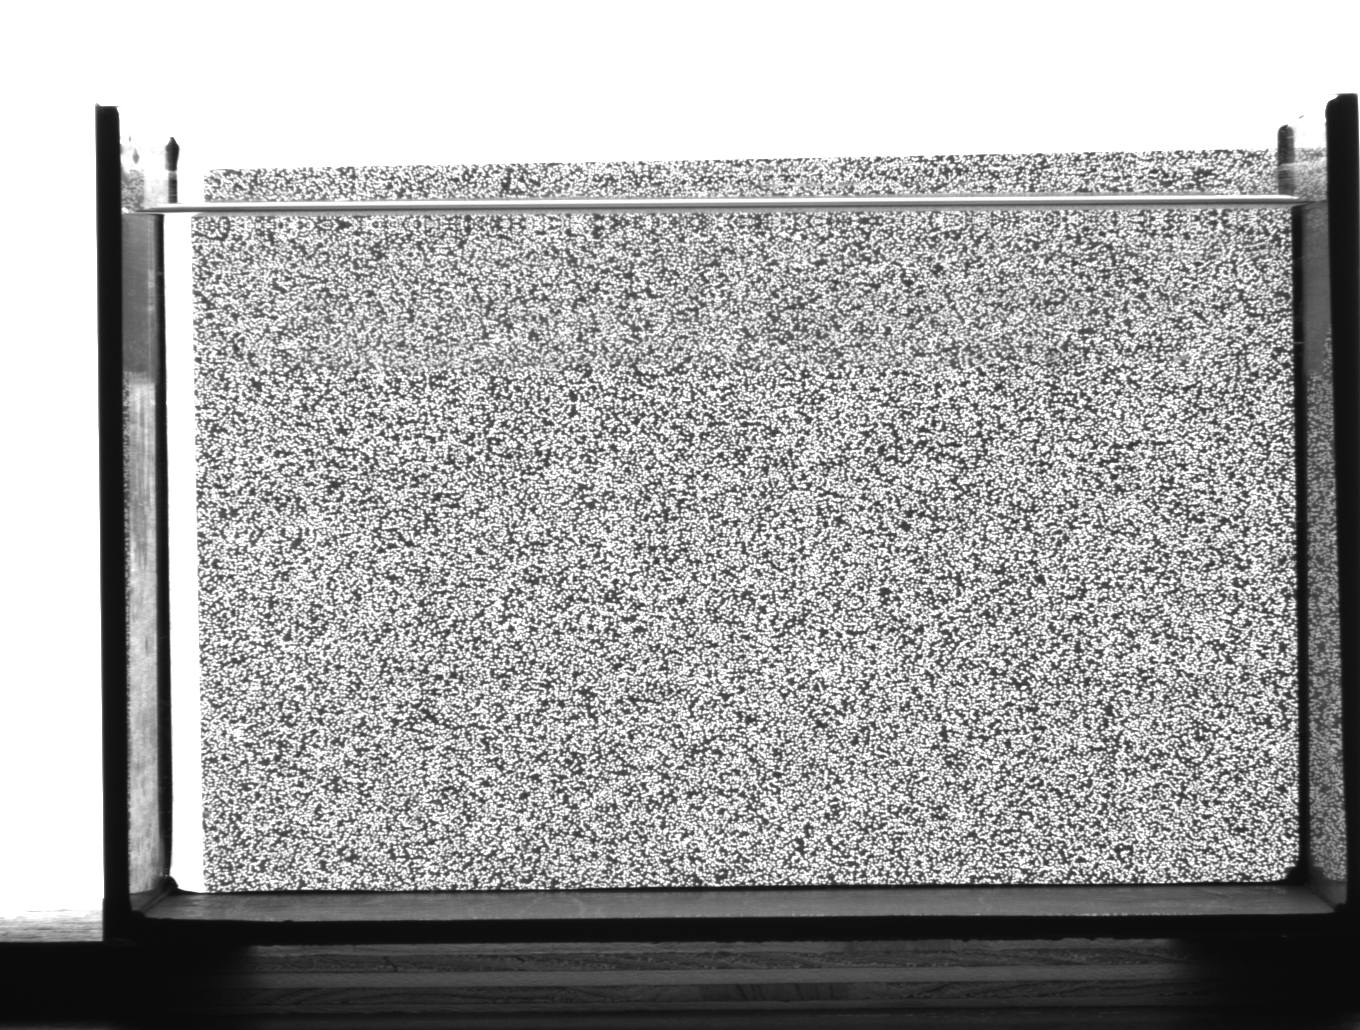
\includegraphics[width = \textwidth,keepaspectratio]{deformedsimplefrontal}
	\subcaption{Deformed Image: Filled with water}\label{fig:fresh0simplefrontal}
\end{subfigure}\\
\begin{subfigure}{.45\linewidth}
	\centering 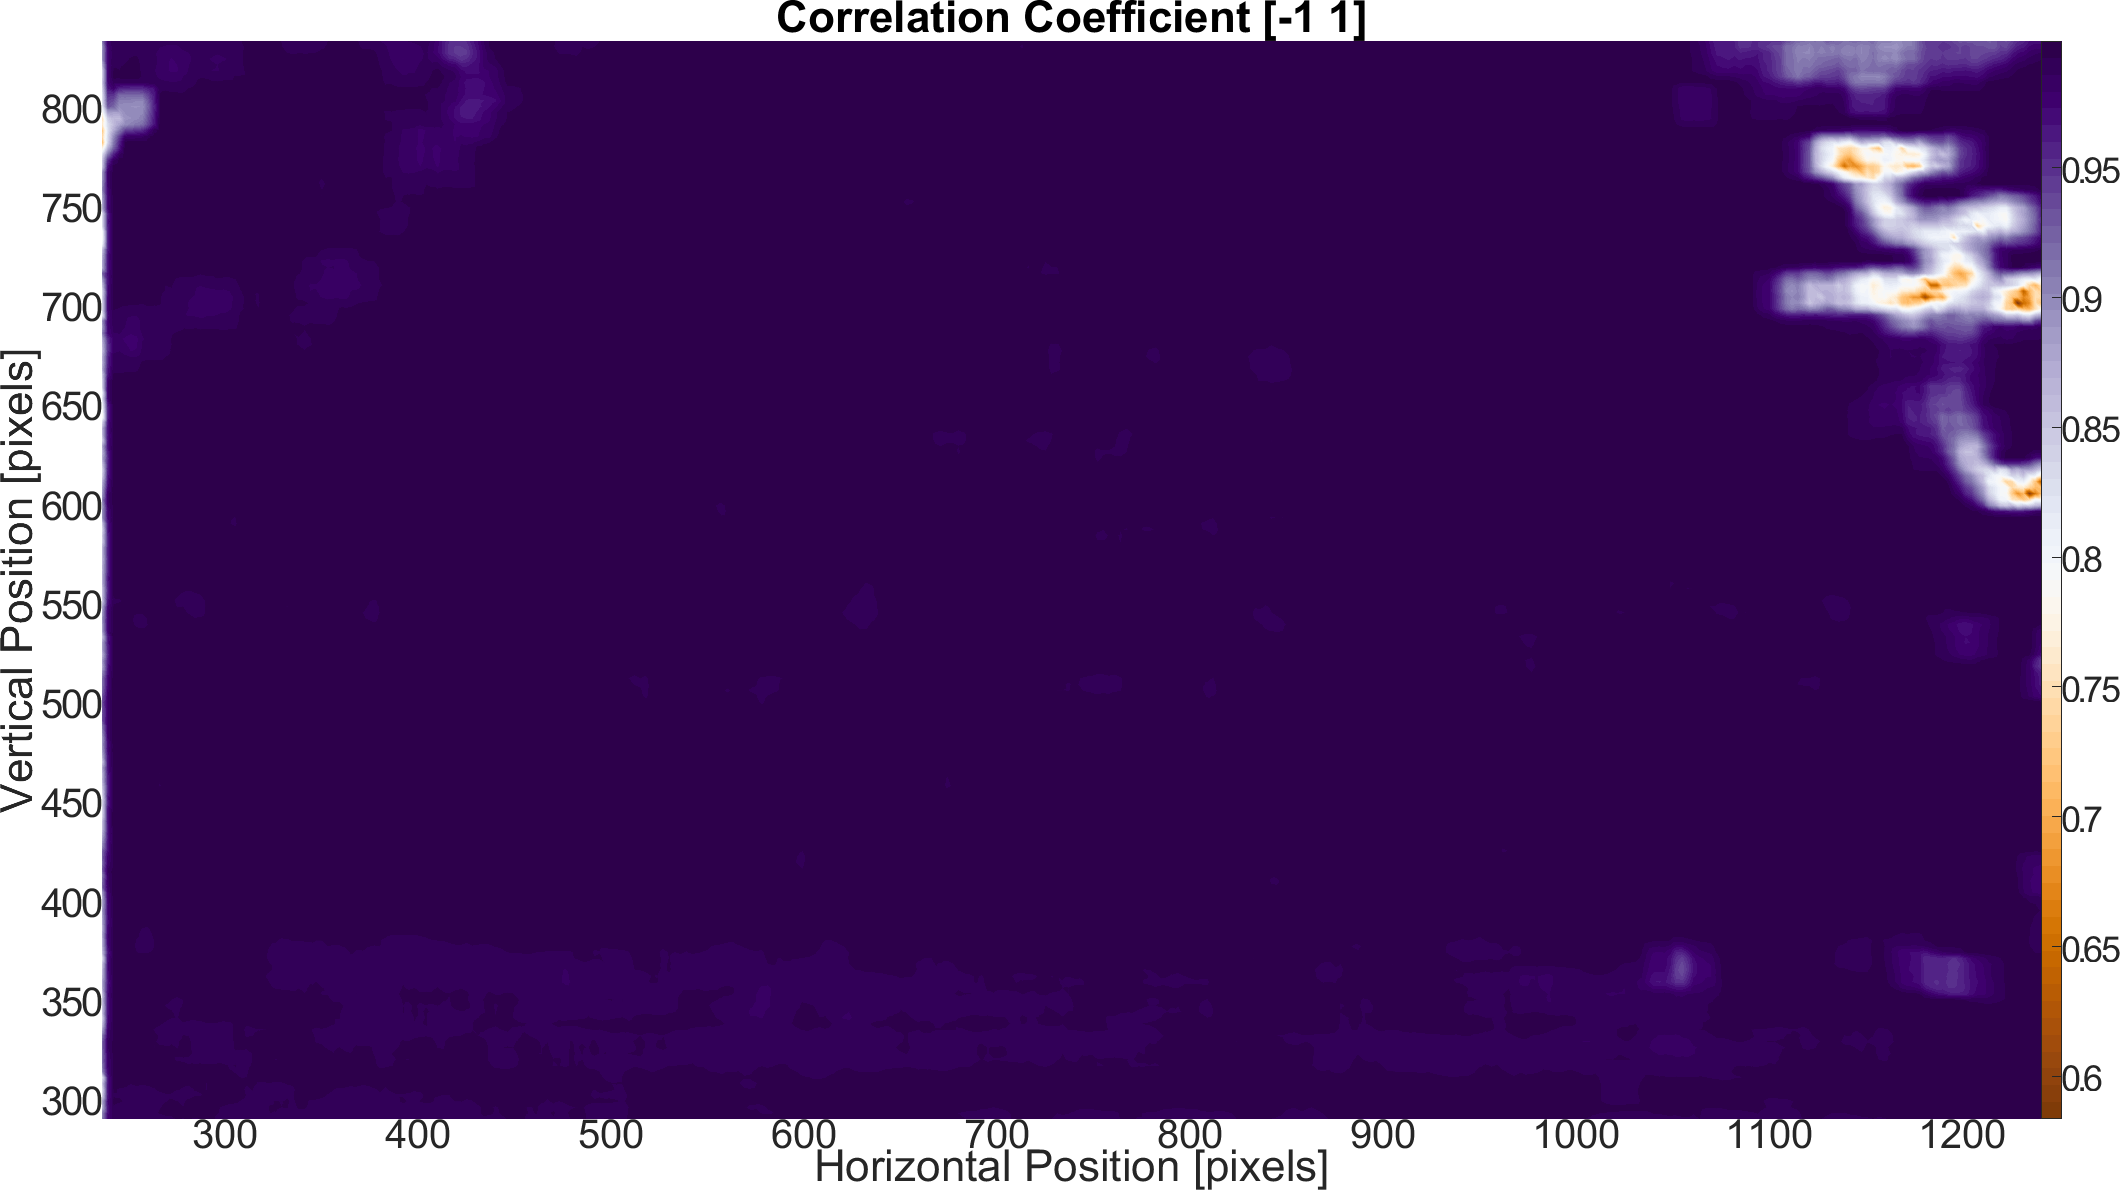
\includegraphics[width = \textwidth,keepaspectratio]{CCsimplefrontal}
	\subcaption{Correlation coefficient from DIC}\label{fig:CCsimplefrontal}
\end{subfigure}%
\begin{subfigure}{.45\linewidth}
	\centering 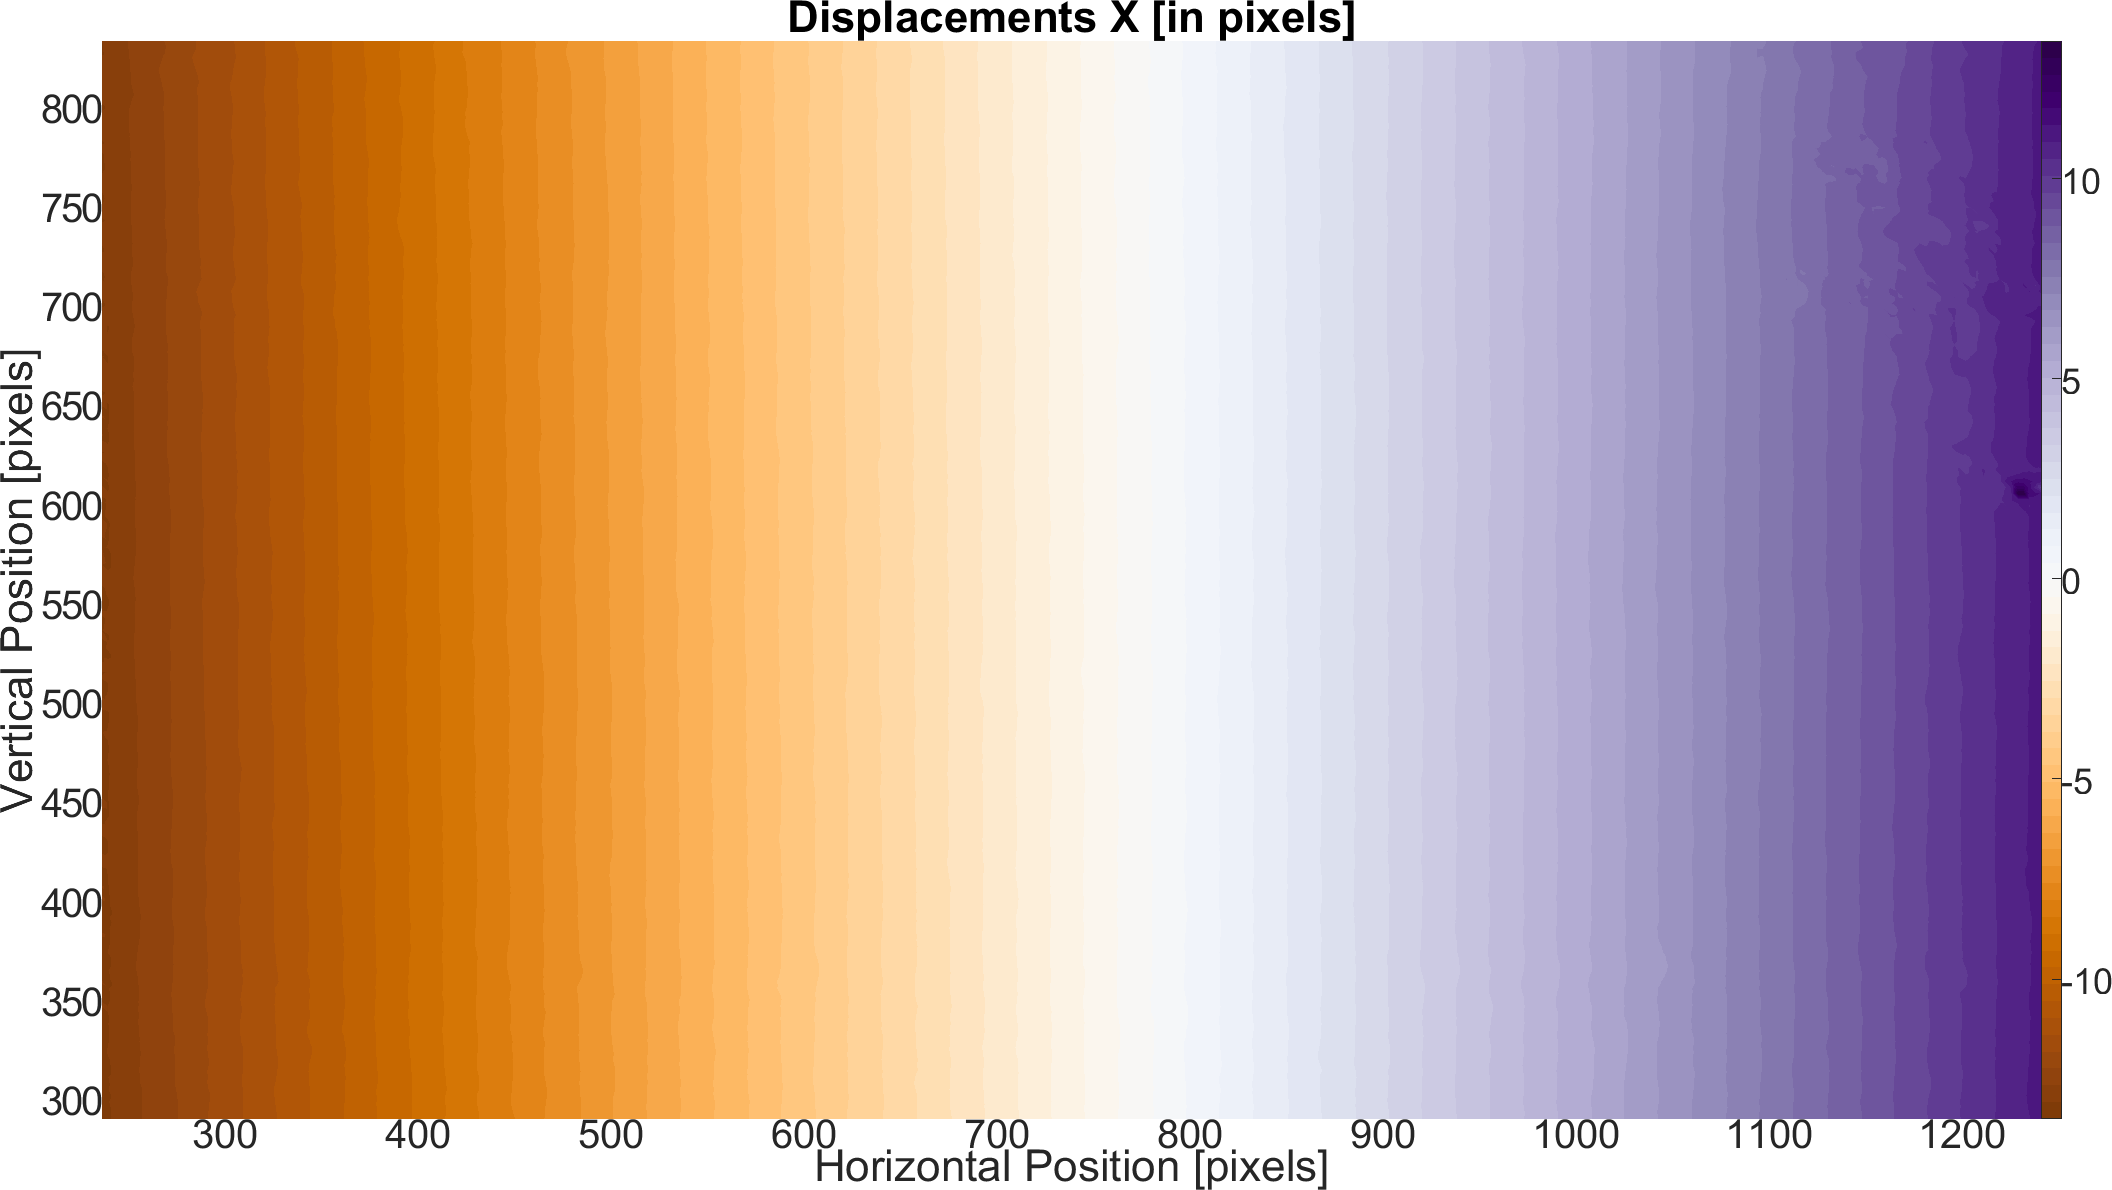
\includegraphics[width = \textwidth,keepaspectratio]{DXsimplefrontal}
	\subcaption{$\Delta x$ from DIC}\label{fig:DXsimplefrontal}
\end{subfigure}\\
	\begin{subfigure}{.45\linewidth}
	\centering 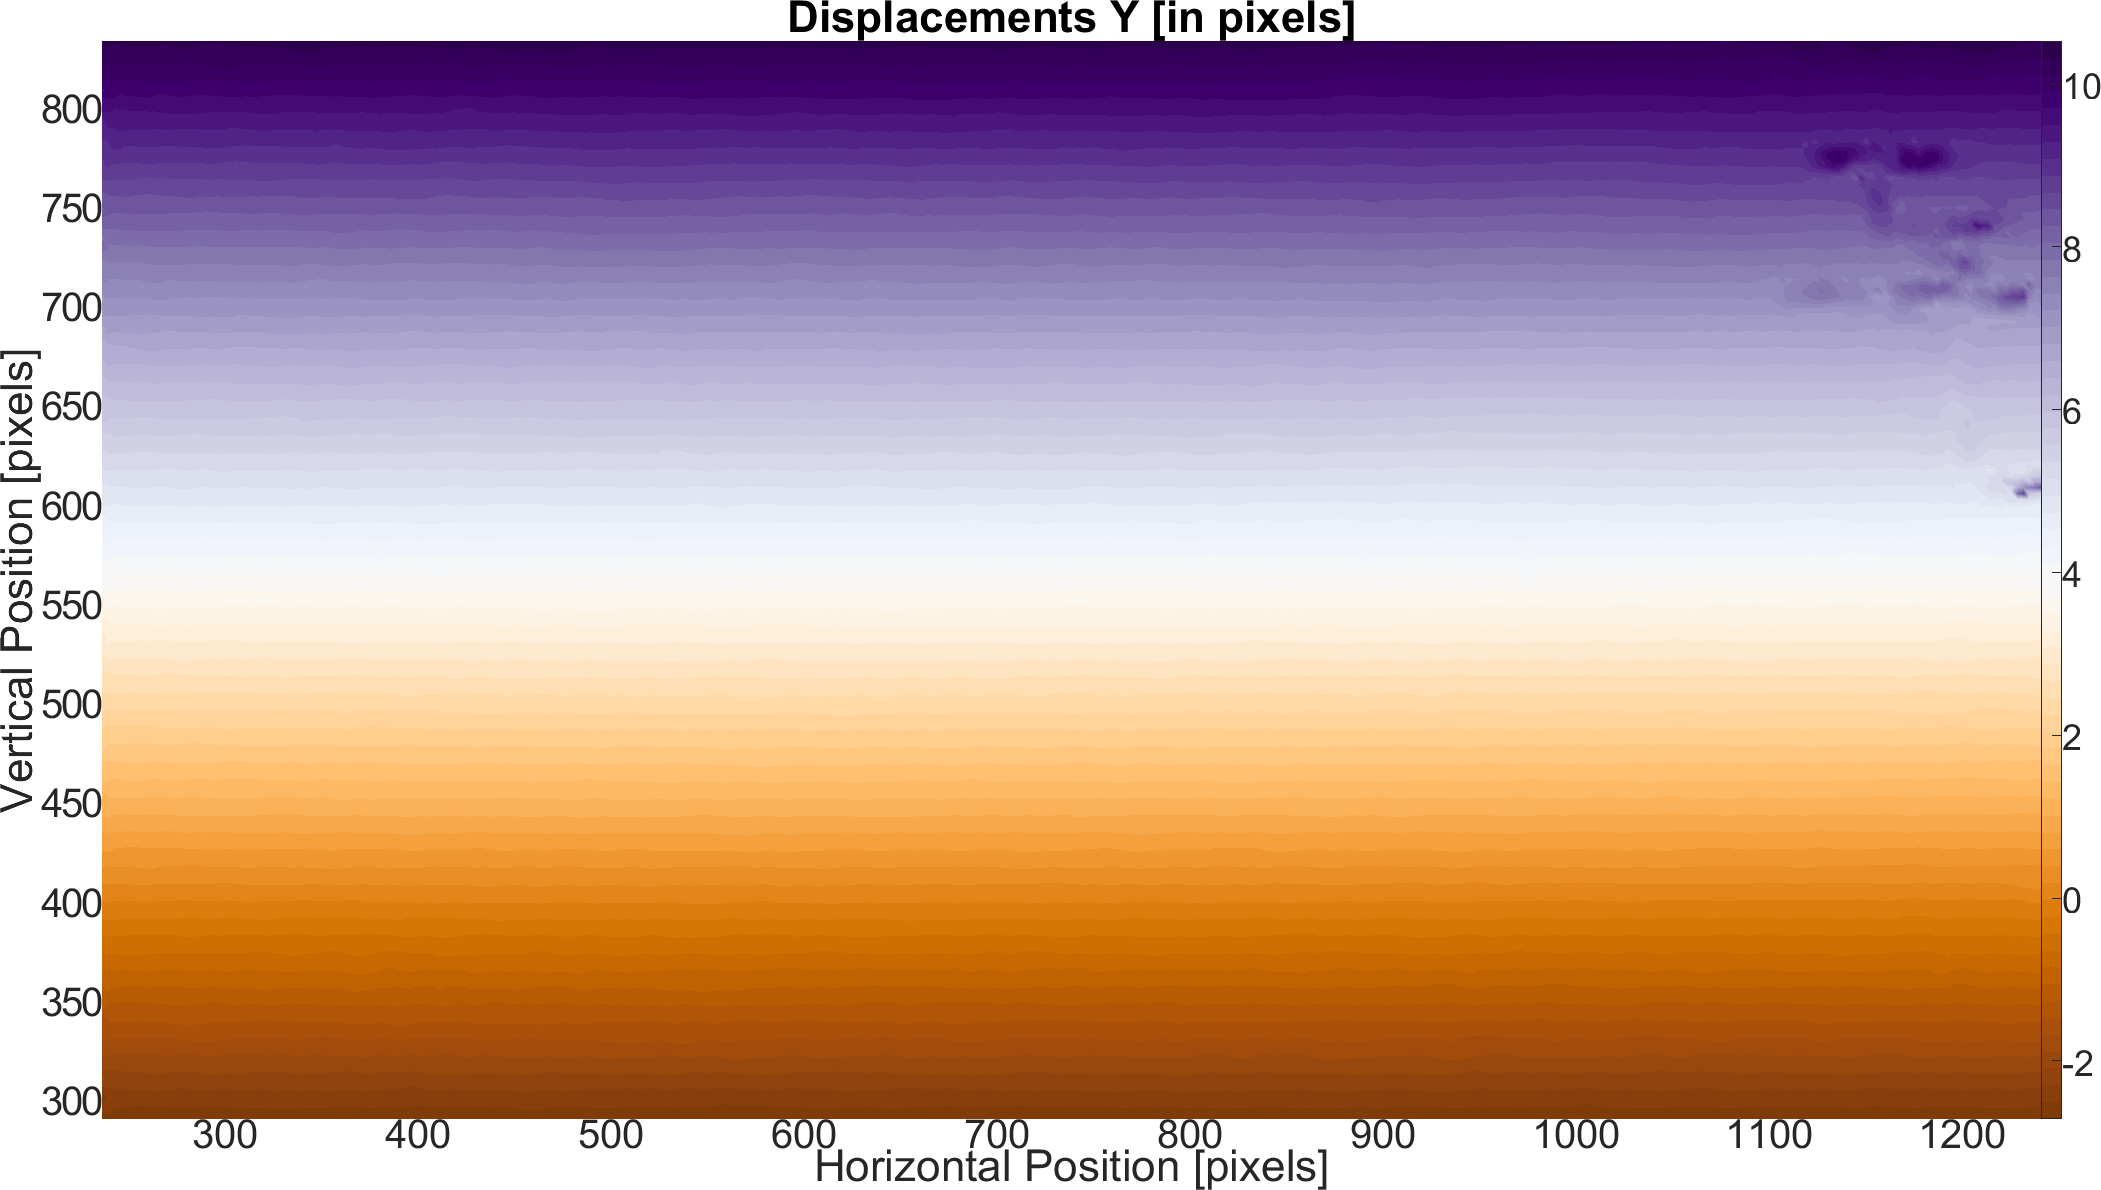
\includegraphics[width = \textwidth,keepaspectratio]{DYsimplefrontal}
	\subcaption{$\Delta y$ from DIC}\label{fig:DYsimplefrontal}
\end{subfigure}%
\begin{subfigure}{.45\linewidth}
	\centering 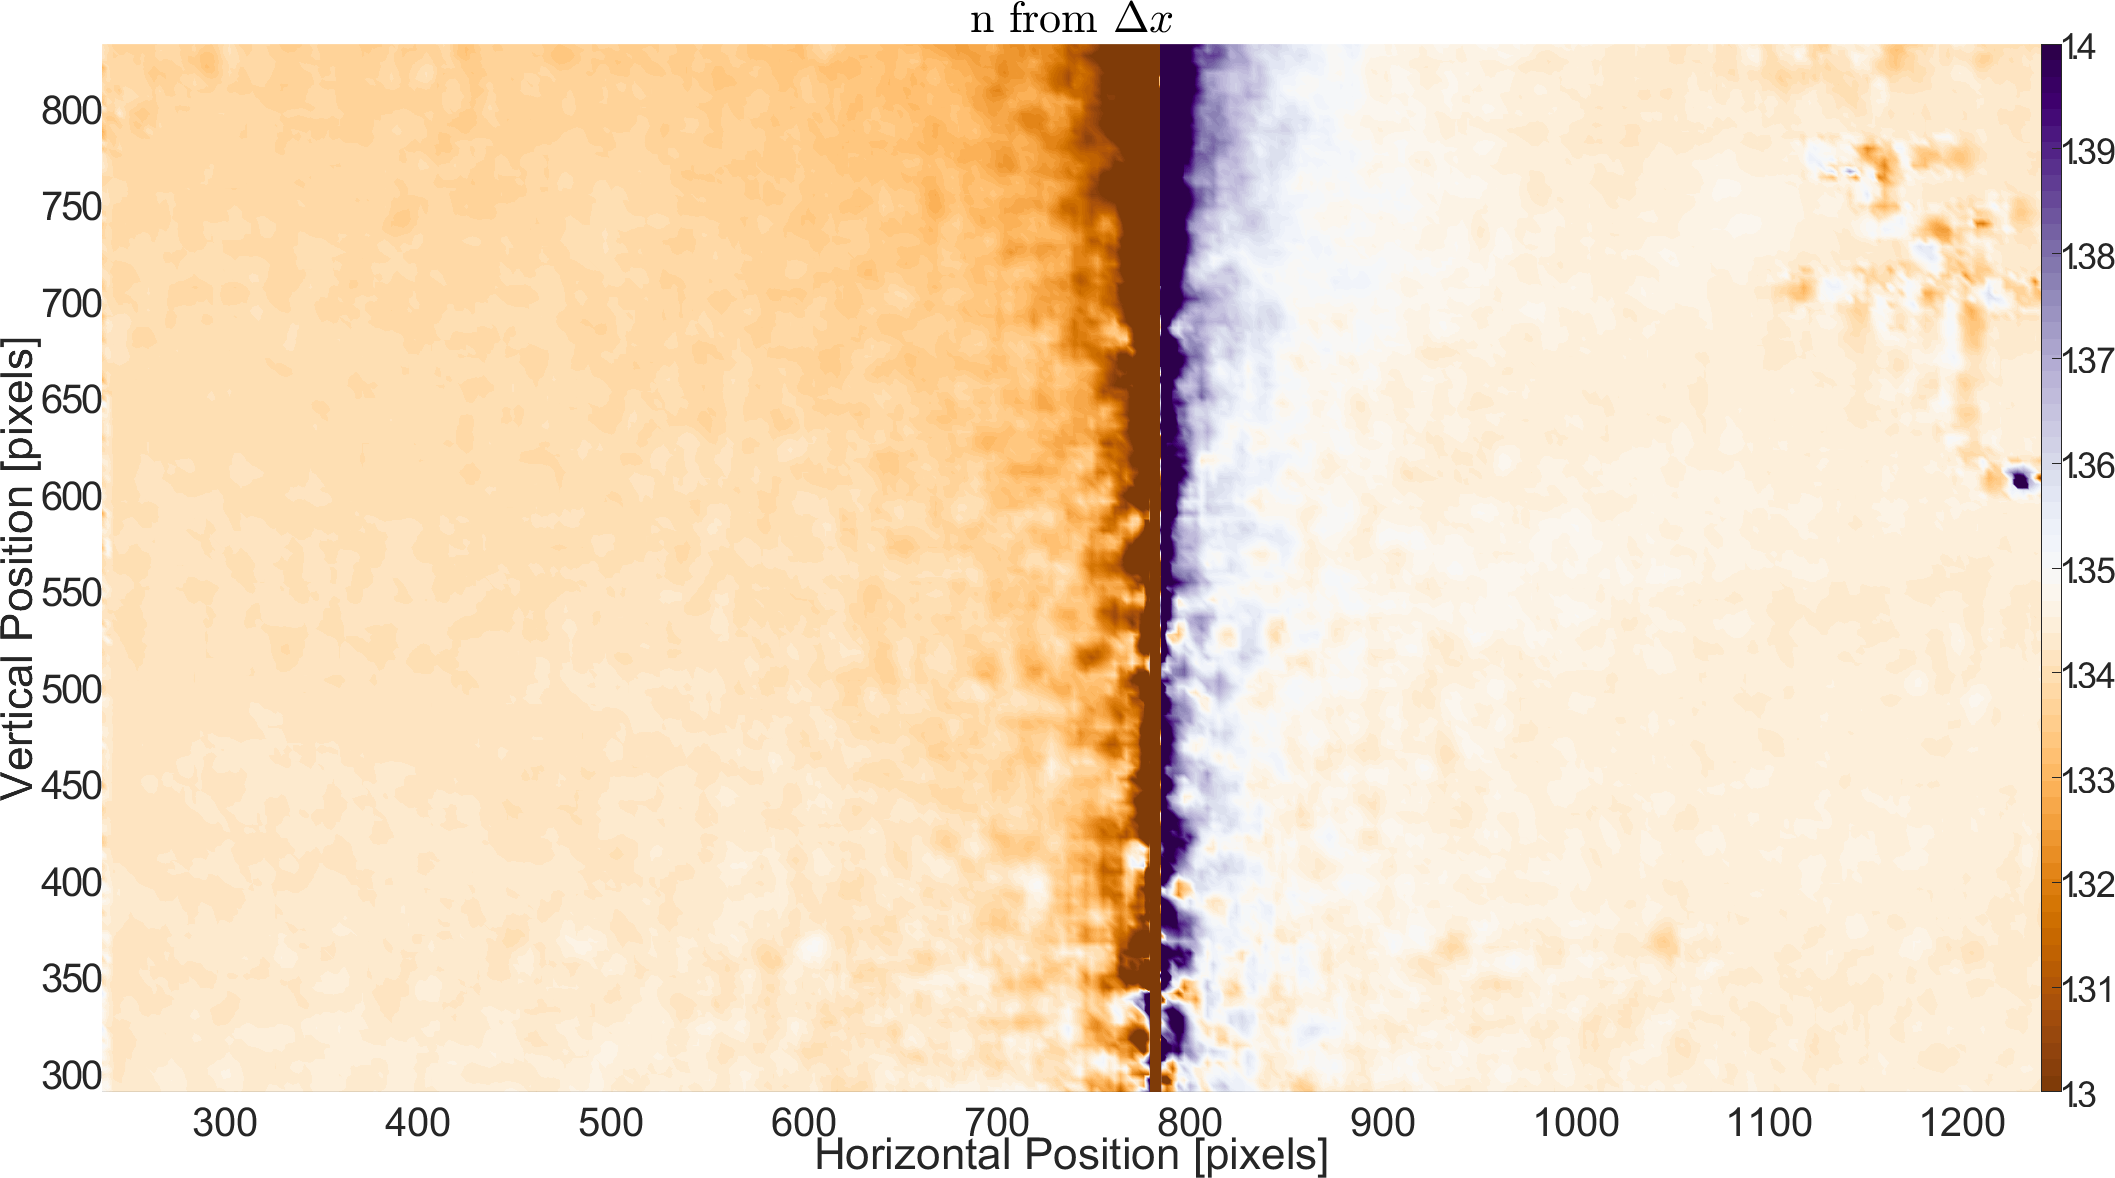
\includegraphics[width = \textwidth,keepaspectratio]{nfromdxsimplefrontal}
	\subcaption{$n$ from $\Delta x$}\label{fig:nfromdxsimplefrontal}
\end{subfigure}\\
\begin{subfigure}{.45\linewidth}
	\centering 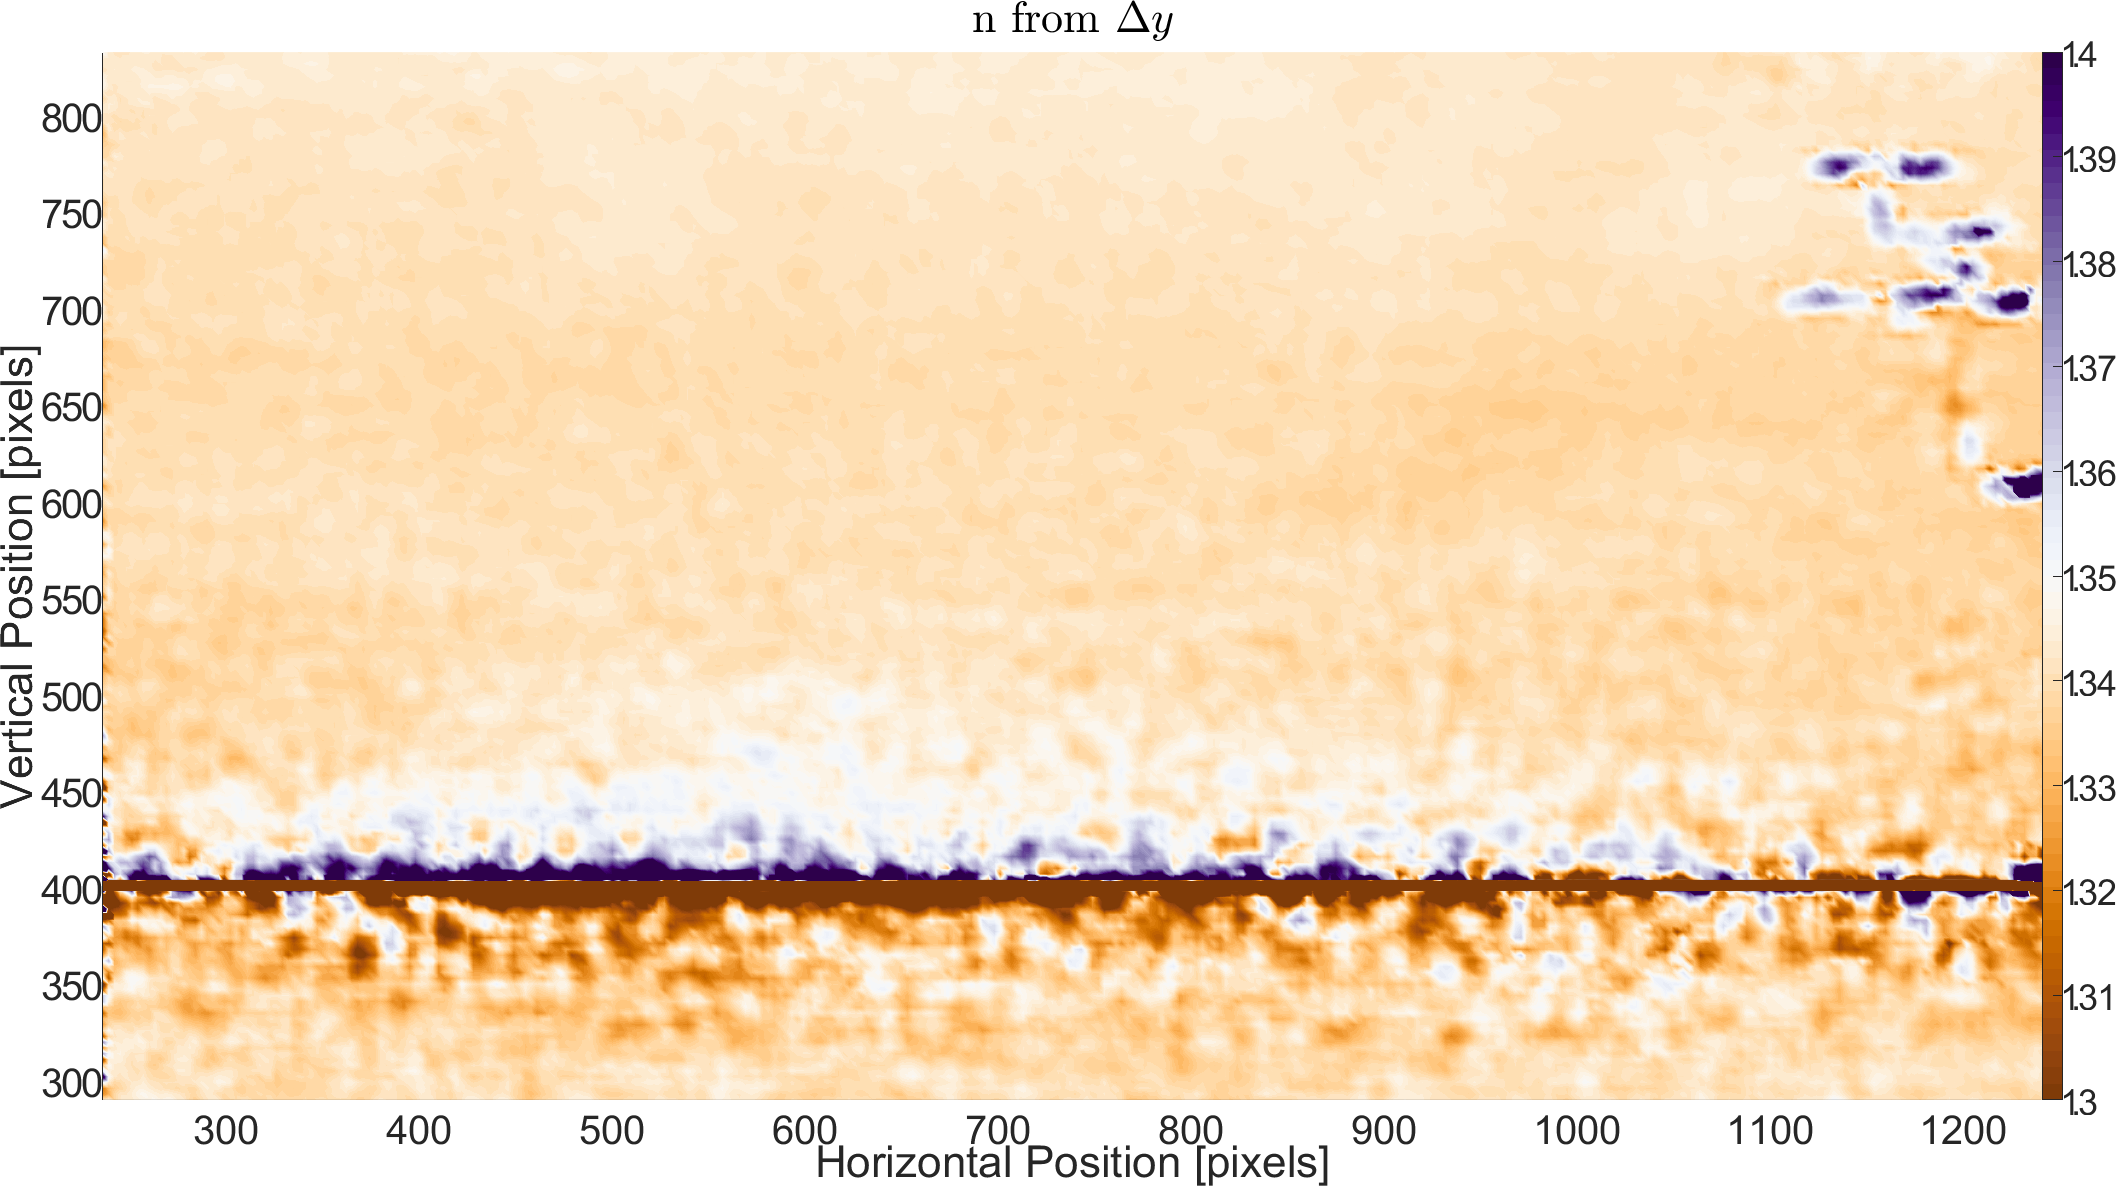
\includegraphics[width = \textwidth,keepaspectratio]{nfromdysimplefrontal}
	\subcaption{$n$ from $\Delta y$}\label{fig:nfromdysimplefrontal}
\end{subfigure}%
\begin{subfigure}{.45\linewidth}
	\centering 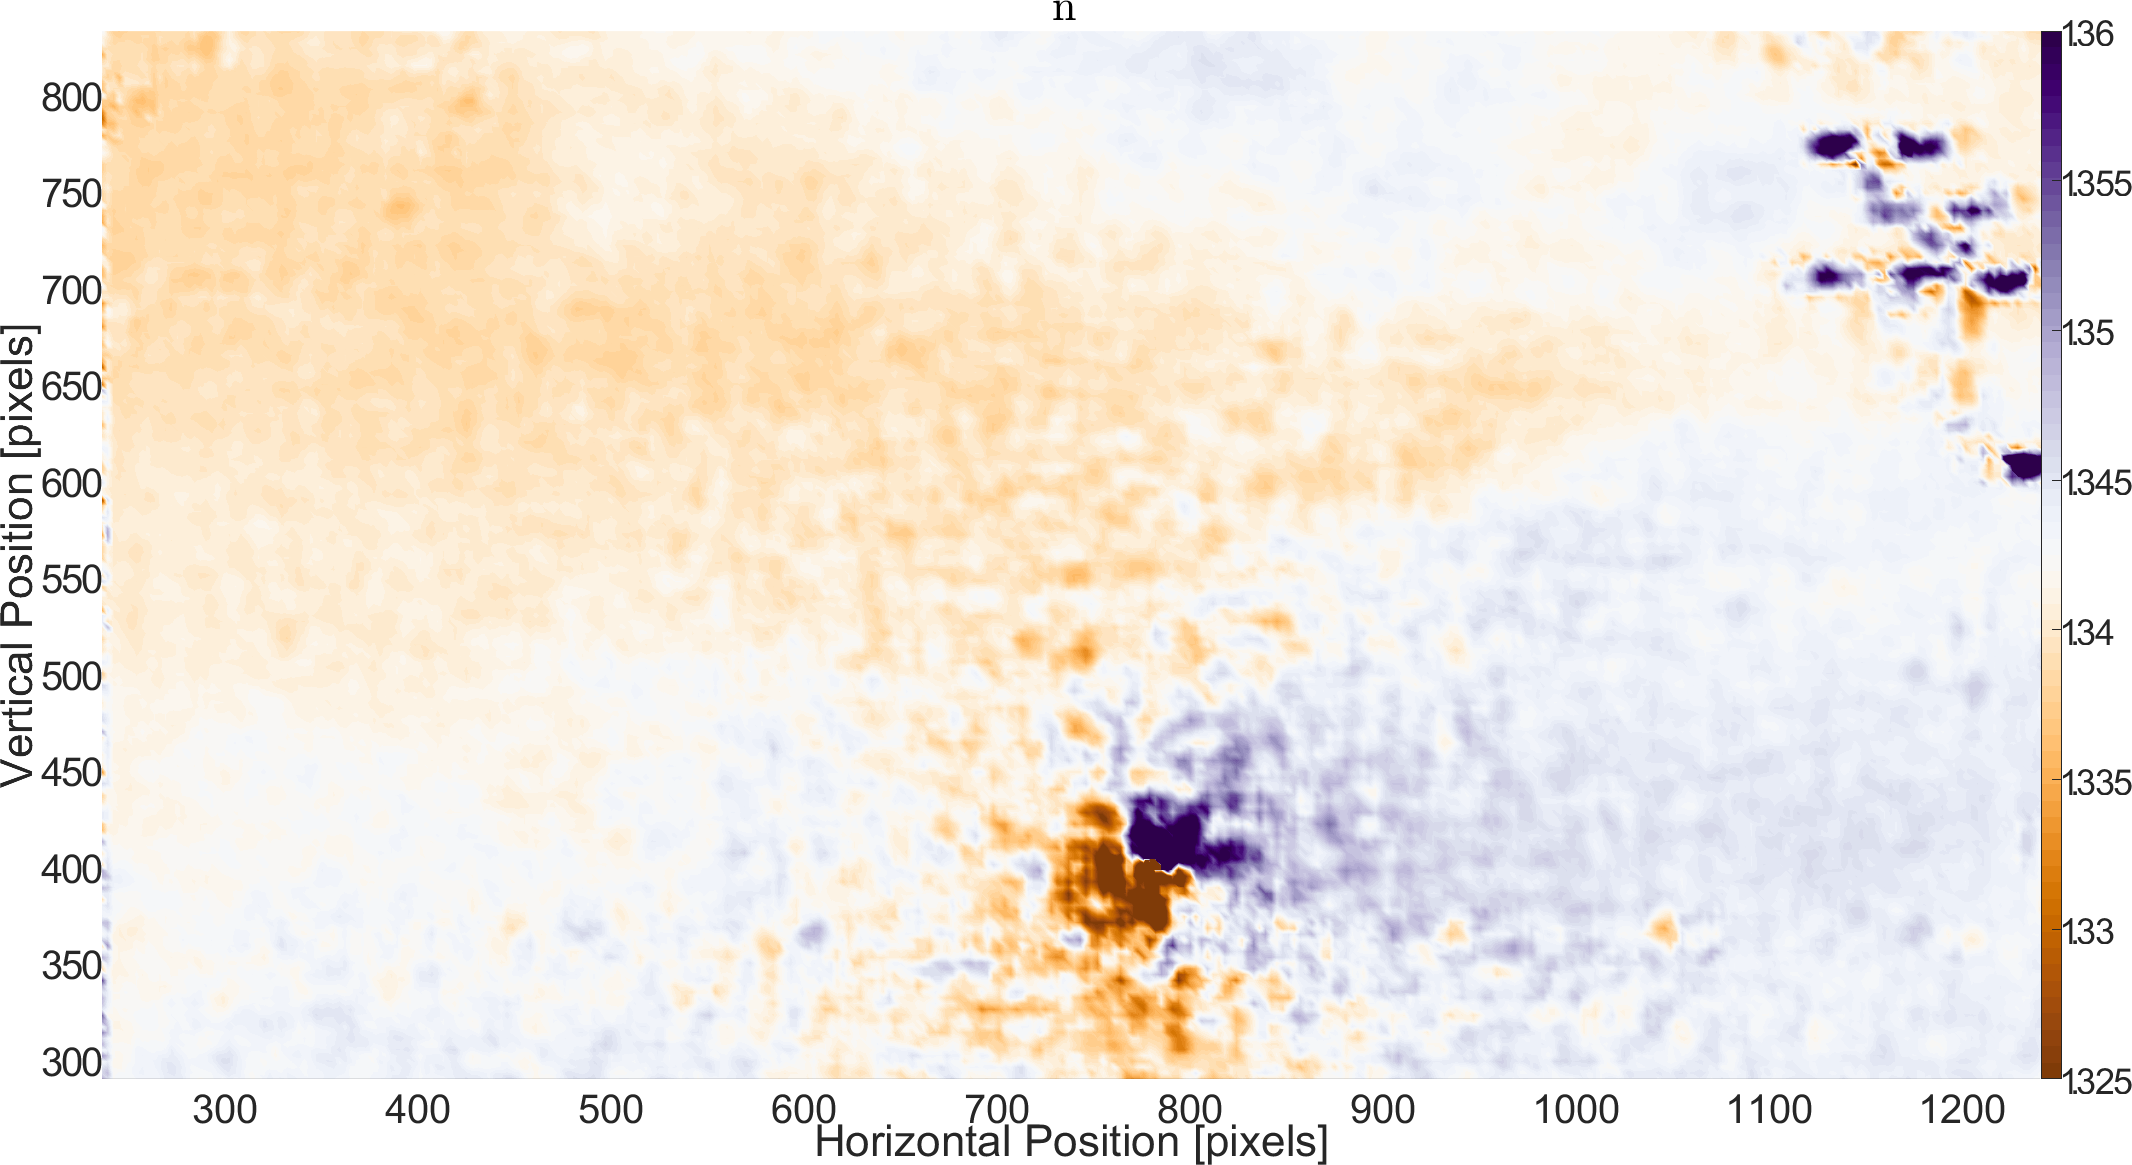
\includegraphics[width = \textwidth,keepaspectratio]{nsimplefrontal}
	\subcaption{$n$ from $\sqrt{\Delta x^2+\Delta y^2}$}\label{fig:nfrontal}
\end{subfigure}
\caption{Simple Model Result. Applying DIC to the Reference Image in \ref{fig:air0simplefrontal} and the Deformed Image \ref{fig:fresh0simplefrontal} yields the correlation coefficient in \ref{fig:CCsimplefrontal}, the horizontal displacements in \ref{fig:DXsimplefrontal} and the vertical displacements in \ref{fig:DYsimplefrontal}. Using (\ref{eq:invdexcon2}) the index of refraction $n$ in \ref{fig:nfromdxsimplefrontal}, \ref{fig:nfromdysimplefrontal} and \ref{fig:nfrontal} are obtained. When the displacements $\Delta x$ and $\Delta y$ approach zero, large errors in $n$ appear. }
\label{fig:simmod}
\end{figure} %Around the location of the $z$-axis, where the angles and displacements approach zero, the errors are large.   and we get possibly negative values of $n$ since both terms in the denominator can go to zero

We see that when the displacements approach zero, we have large errors in $n$. Figure \ref{fig:nfrontal} looks best, but is still unacceptable.The entire figure should have a constant value of $n = 1.333$. This is not the case.
 
Equations (\ref{eq:dexcon2}) and (\ref{eq:invdexcon2}) reveal a problem when determining $n$: When the angle $\theta_x$ goes to zero, (\ref{eq:dexcon2}) shows $\Delta x$ goes to zero. Then the numerator in the fraction in (\ref{eq:invdexcon2}) goes to zero, while the two terms in the denominator both go to zero. So we get large errors in the magnitude of $n$ since we are dividing $0/0$. In any measurement we have noise, resulting in uncertainties in $\Delta x$ and $\theta_x$. These uncertainties have a large effect on the value of $n$ since the expected values of $\Delta x$ and $\theta_x$ are small. %The Signal-to-Noise Ratio is very bad because our signal is very small.

To solve this, we want $\theta_x$ to not approach zero. Then, according to (\ref{eq:dexcon2}), $\Delta x$ does not approach zero and our calculation of $n$ is not plagued by a fraction that approaches $0/0$. To achieve this, we place our camera at an angle $\alpha$ with respect to the water tank. The angle $\theta_x$ is replaced by $\alpha+\phi_x$, where $\phi_x$ is the angle of the light ray relative to the principal axis of the camera, which is at an angle $\alpha$. %For example, we position our camera at an angle of $\alpha=30^\circ$ relative to the tank. The camera has a viewing range of $[-4,4]^\circ$. Then $\phi_x$ varies from $-4^\circ$ to $4^\circ$.

%\begin{figure}[hpbt]
%	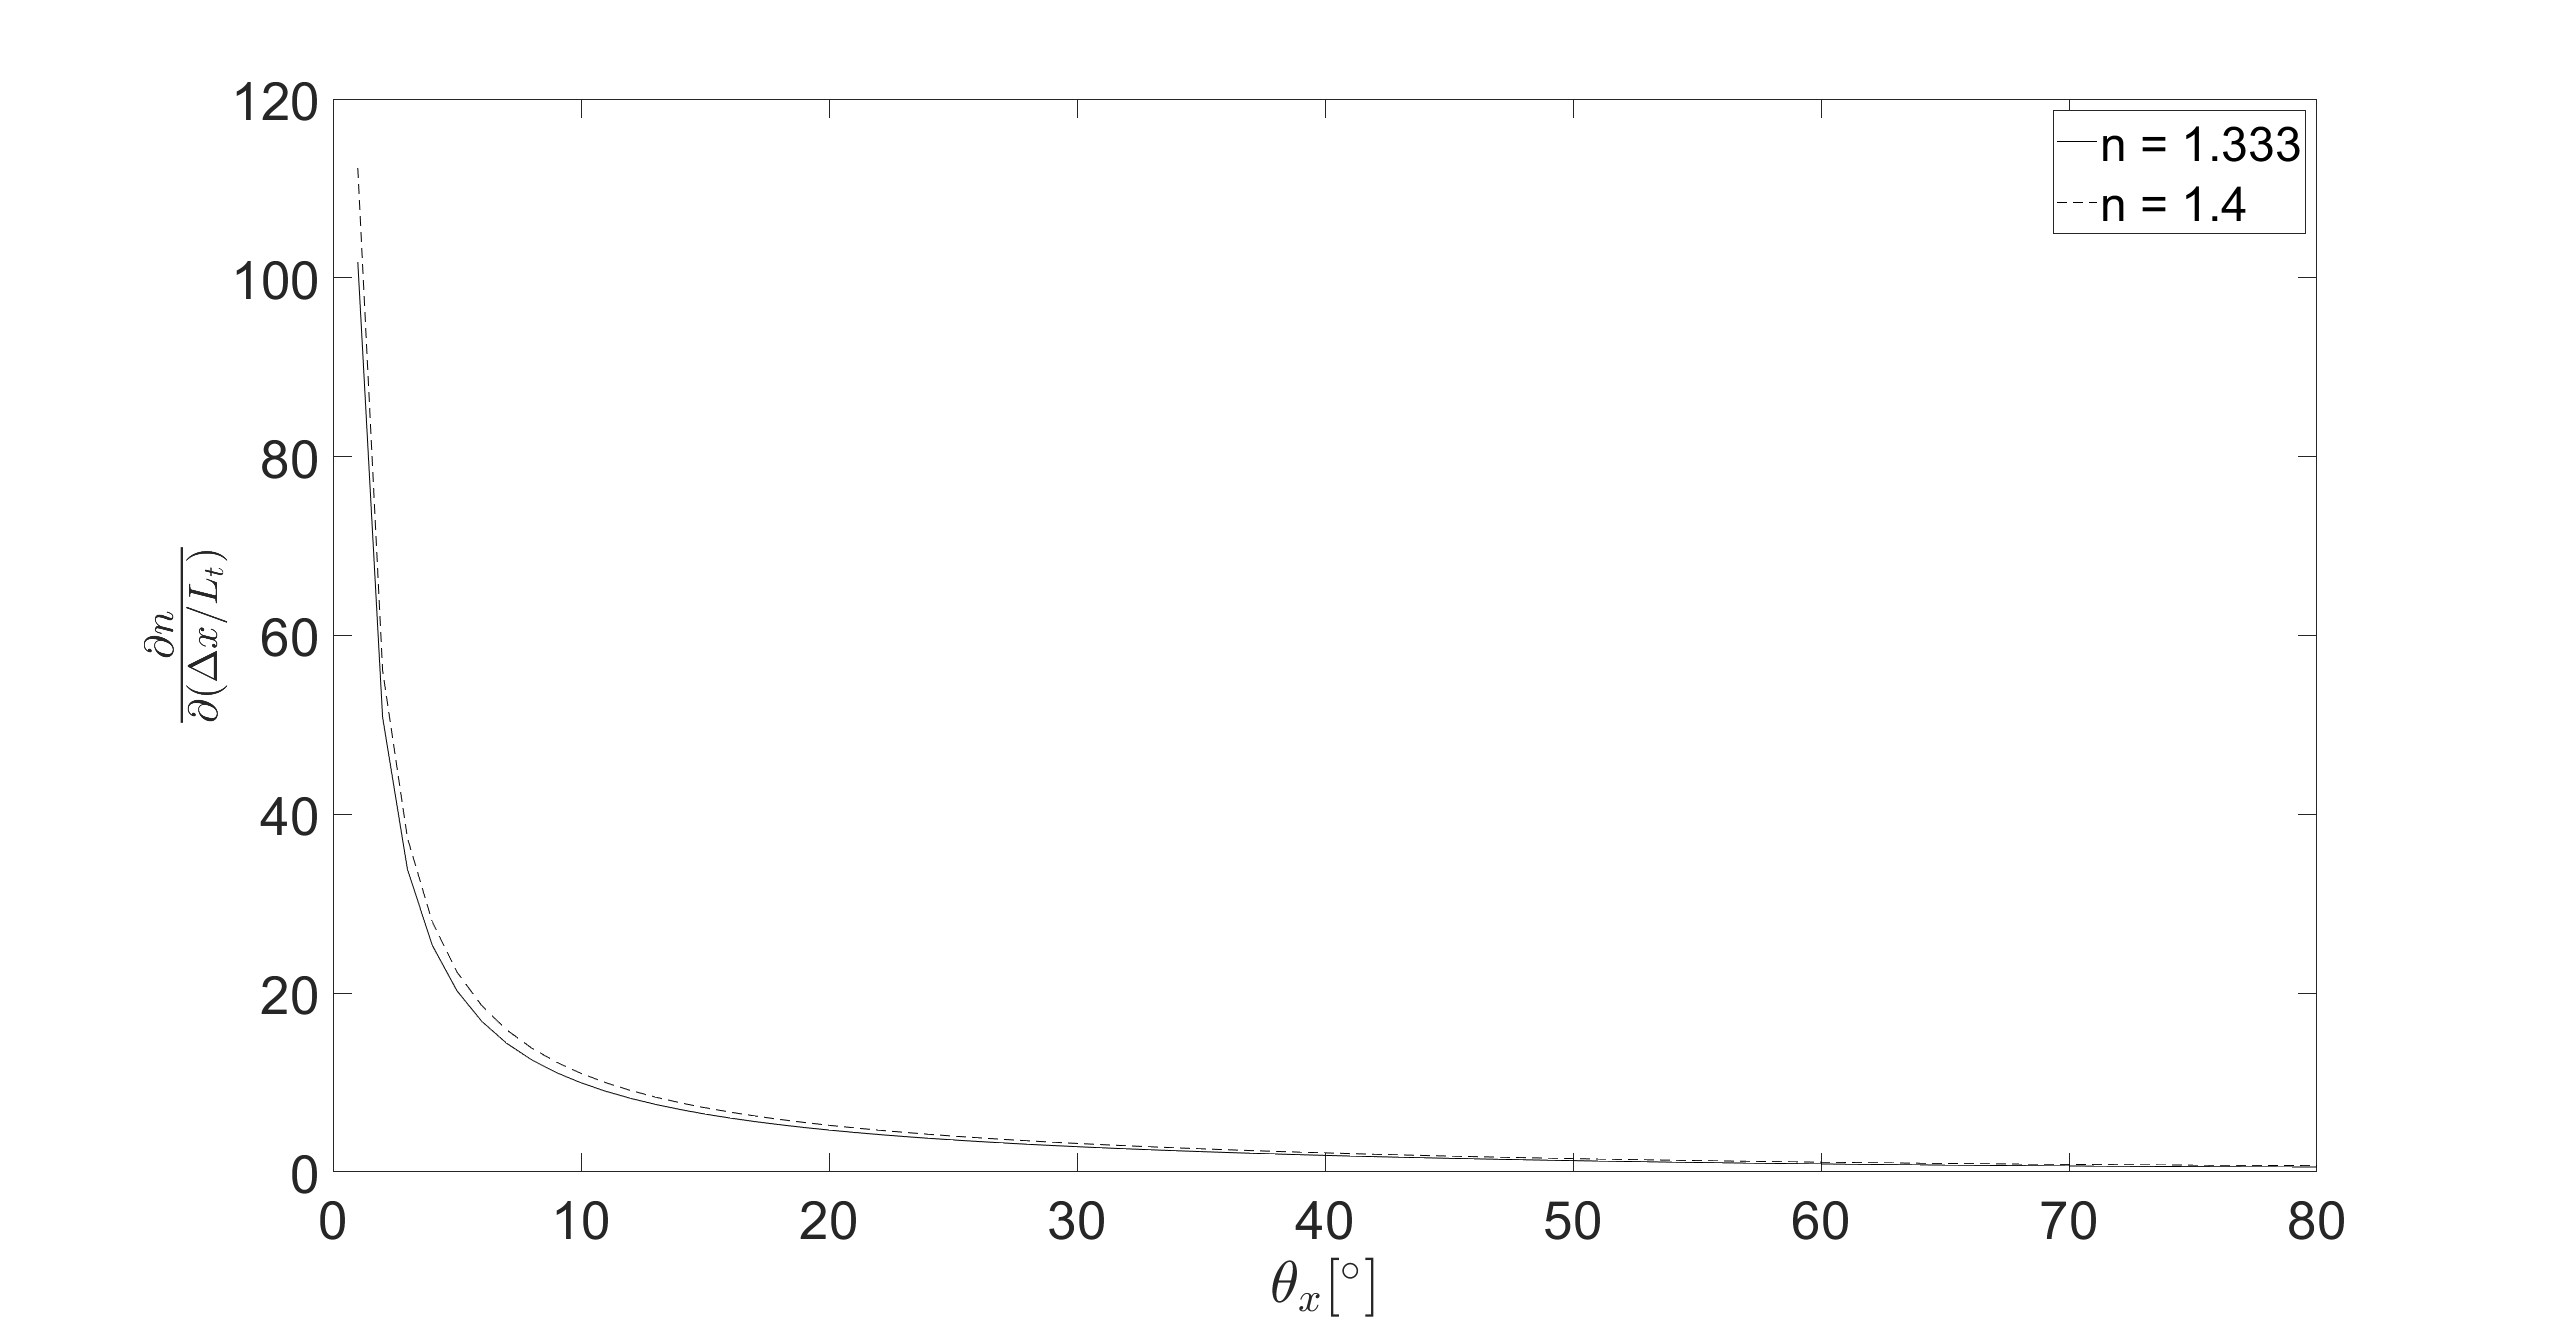
\includegraphics[width=\textwidth, keepaspectratio]{dndx.png}
%	\caption{Derivative of $n$ with respect to $\Delta x / L_t$ as a function of $\theta_x$.}	
%	\label{fig:dndx}
%\end{figure}
%
%\begin{figure}[hpbt]
%	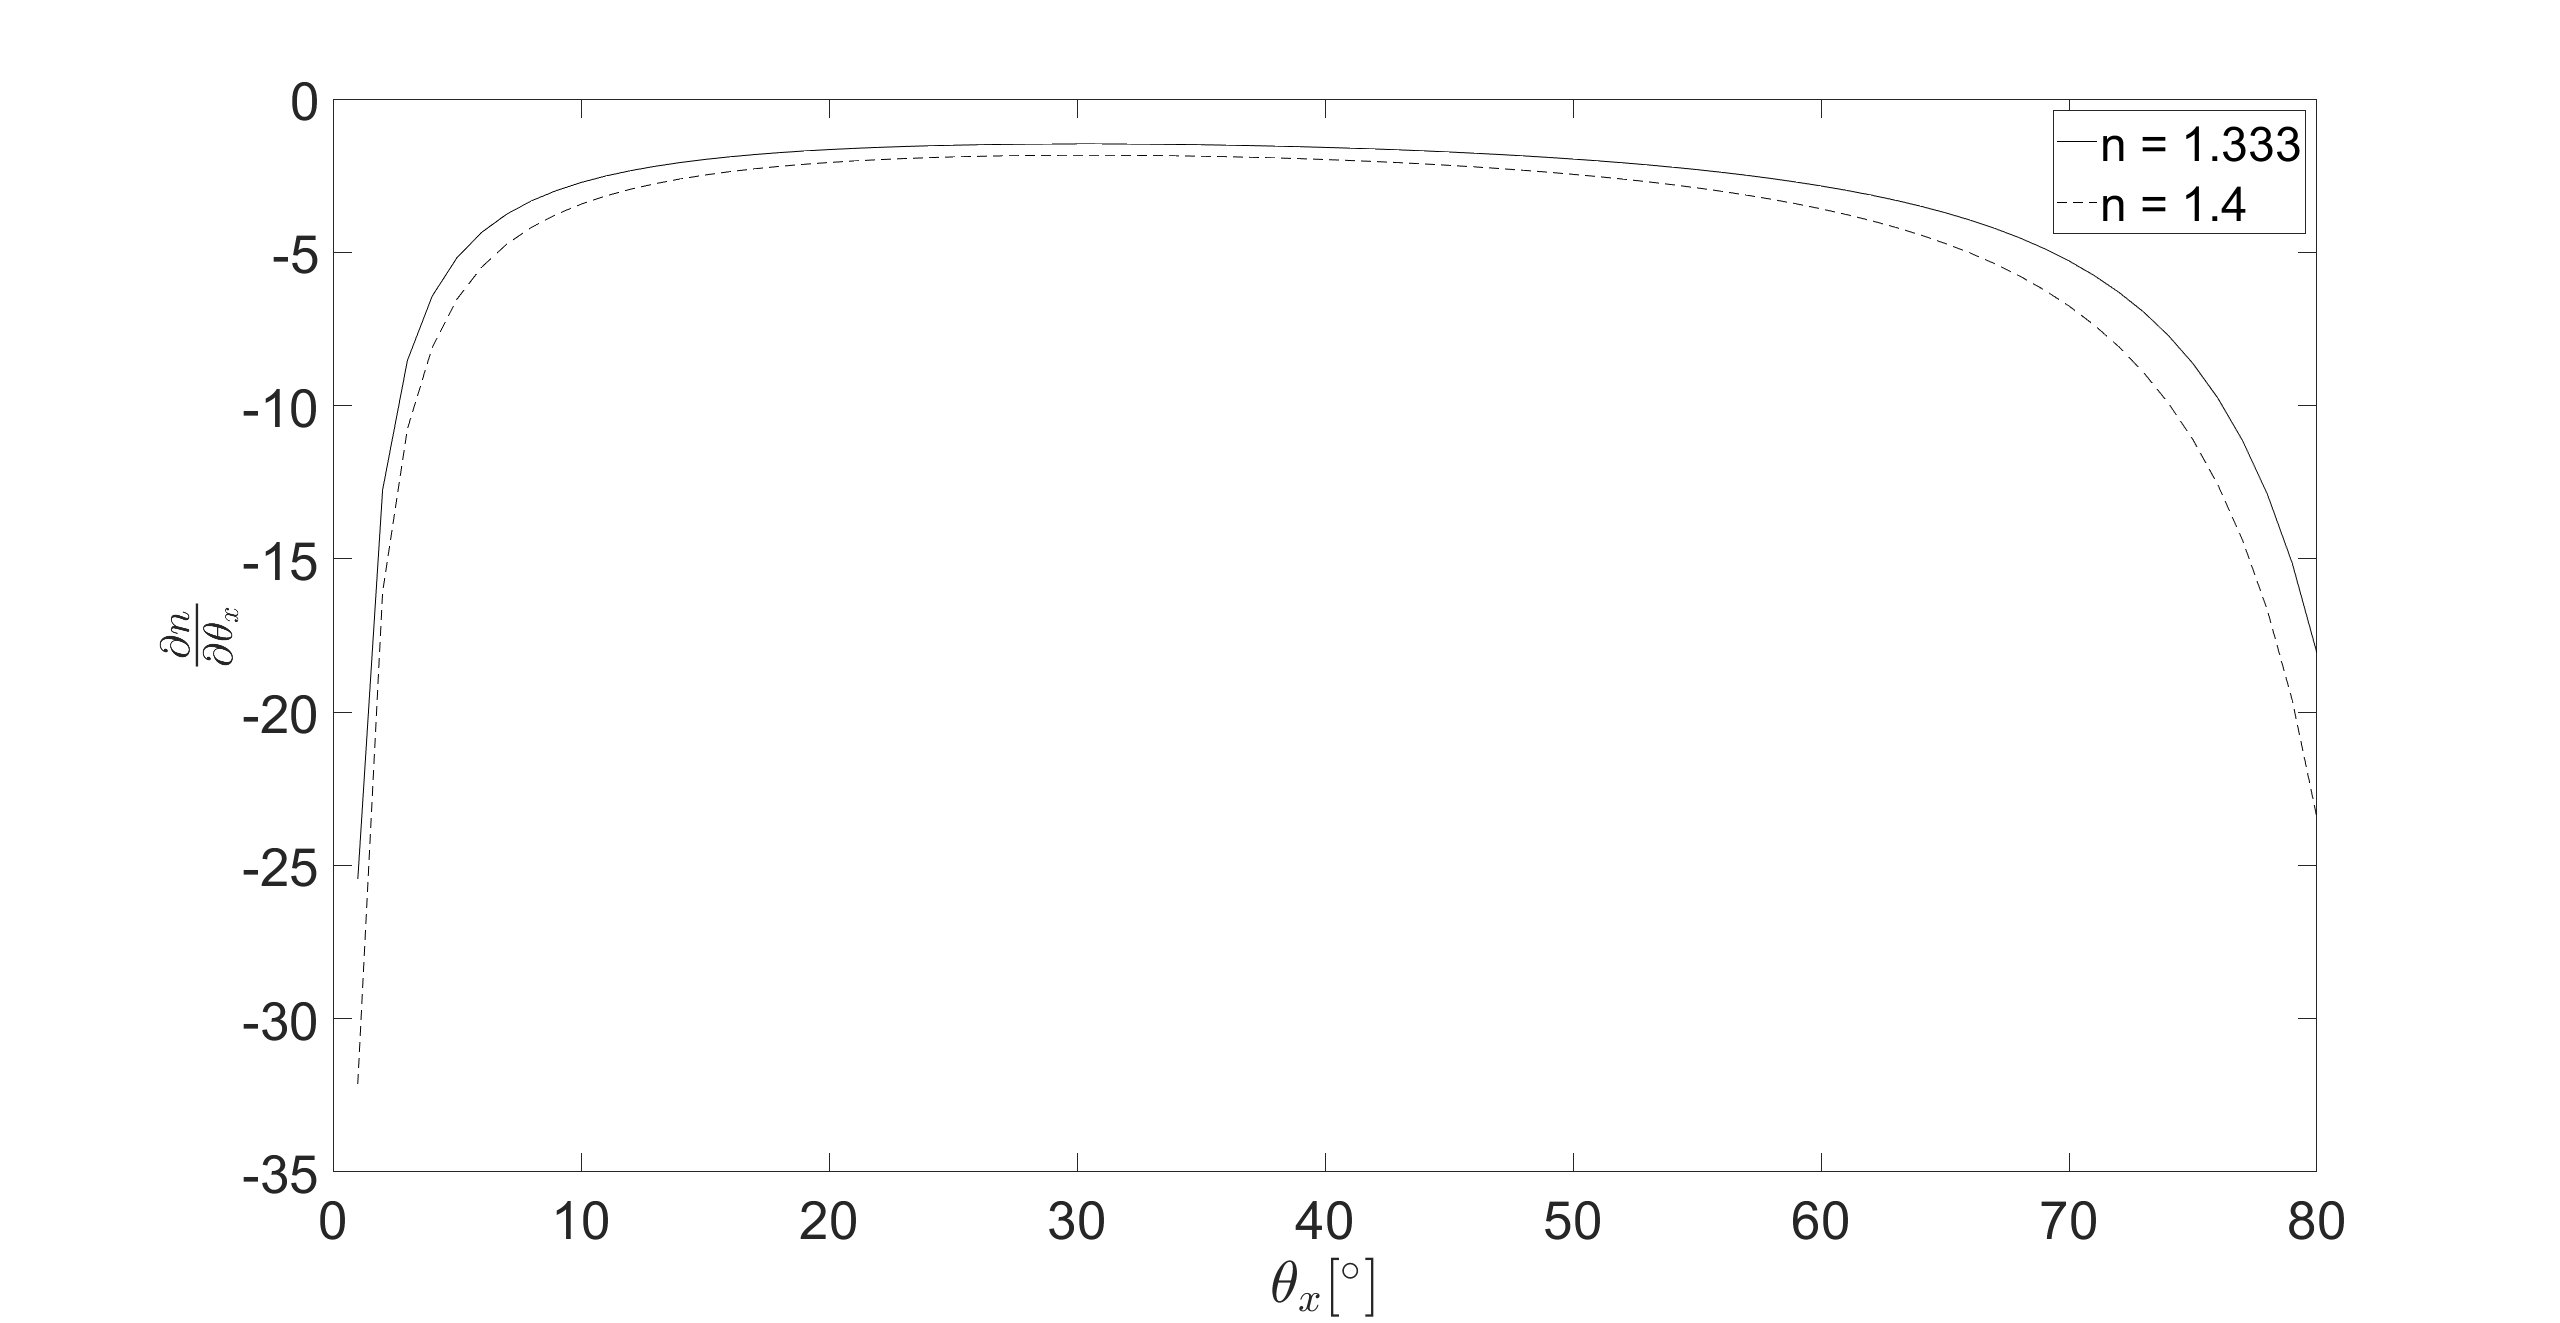
\includegraphics[width=\textwidth, keepaspectratio]{dndt.png}
%	\caption{Derivative of $n$ with respect to $\theta_x$ as a function of $\theta_x$.}		
%	\label{fig:dndt}
%\end{figure}

\begin{figure}[hpbt]
	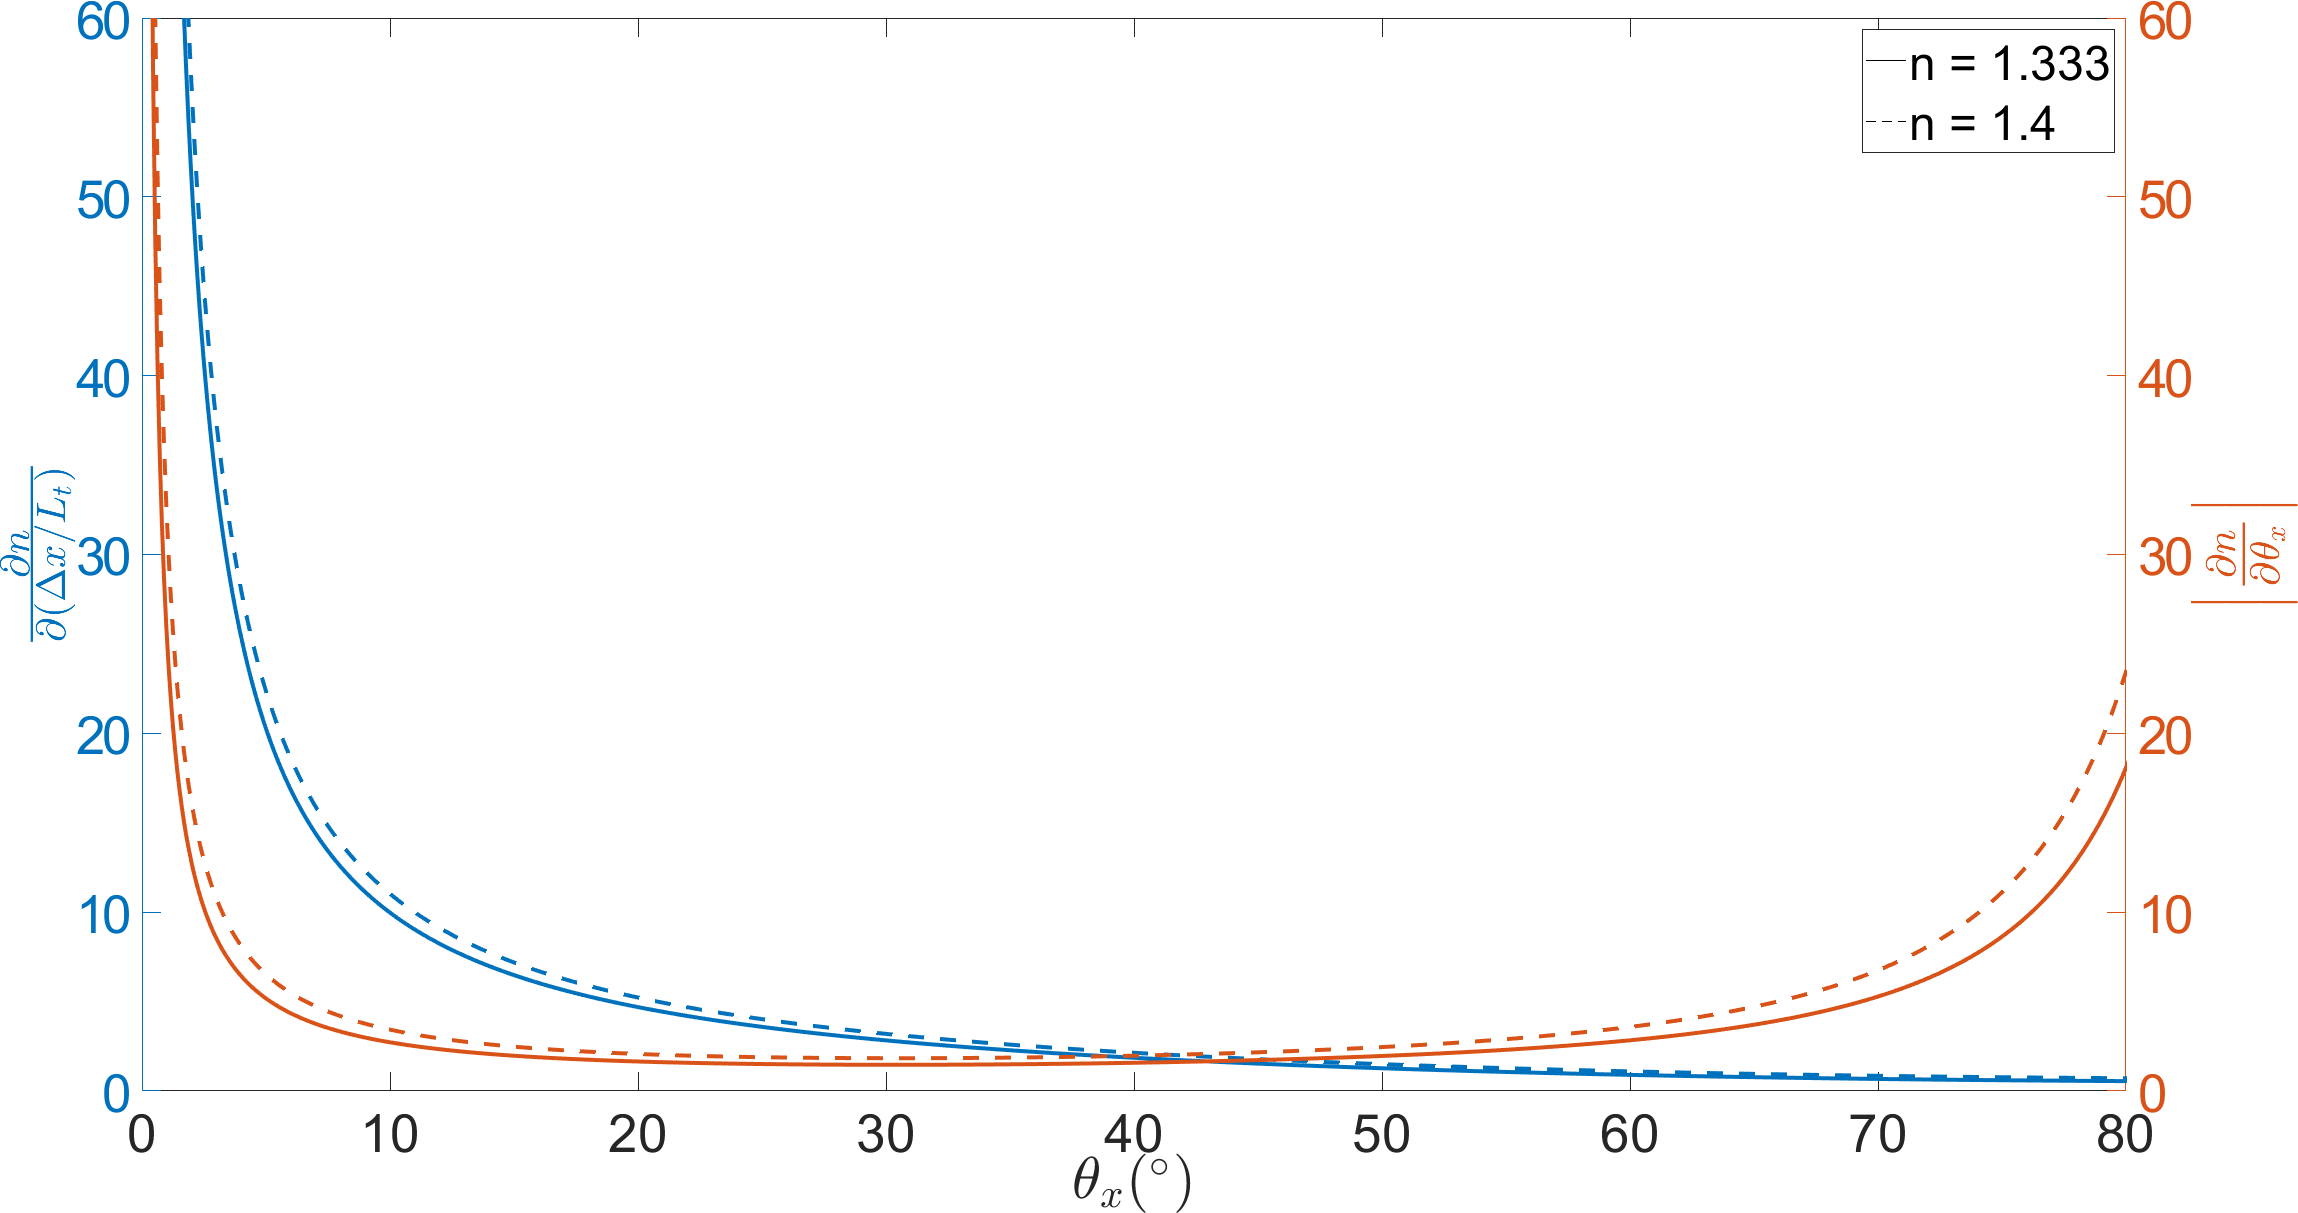
\includegraphics[width=\textwidth, keepaspectratio]{diffnsimple.png}
	\caption{Derivative of $n$ with respect to $\Delta x / L_t$ and $\theta_x$ as a function of $\theta_x$.}		
	\label{fig:diffnsimple}
\end{figure}

We want $\Delta x$ and $\theta_x$ to vary with $n$ as much as possible. So, we want $n$ to vary with $\Delta x$ and $\theta_x$ as little as possible. To find the best angle $\theta_x$ to achieve this, we take the derivative of (\ref{eq:invdexcon2}) with respect to $\Delta x/L_t$ and $\theta_x$ \cite{nemoto1992measurement}. Figure \ref{fig:diffnsimple} shows these derivatives: $\partial n/\partial (\Delta x/L_t)$ decreases with increasing $\theta_x$. $\left|\partial n/\partial \theta_x\right|$ first decreases with increasing $\theta_x$, reaches a minimum, then increases again. The worst possible angle to measure is $0^\circ$. 

%Since there is also an uncertainty in the angle, we want $n$ to vary with $\theta_x$ as little as possible. Figure \ref{fig:diffnsimple} also shows this derivative. The magnitude of this derivative $\left|\partial n/\partial \theta_x\right|$ first decreases with increasing $\theta_x$, reaches a minimum, then increases again. The worst possible angles to measure at are $0^\circ$ and $90^\circ$. The minimum is reached at $31^\circ$. Any angle between $15^\circ$ and $55^\circ$ yields approximately the same sensitivity of $n$. 

%Viewing at too large an angle (e.g. $70^\circ$) makes it hard to see through the water tank. 
%As an example, we take an index of refraction $n=1.333$, an index of refraction $n_0 = 1$, a tank width $L_t=0.2[m]$ and an angle $\theta_x=30^\circ$. (\ref{eq:dexcon2}) yields a $\Delta x = 0.0345[m]$. From Figure (\ref{fig:dndx}), $\partial n/\partial (\Delta x/L_t) = 2.831$  at $\theta_x = 30^\circ$. Hence an error of $1[mm]$ in $\Delta x$ causes an error of $0.014$ in $n$. From Figure (\ref{fig:dndt}), $\partial n/\partial \theta_x = -1.466$  at $\theta_x = 30^\circ$. Hence an error of $0.1^\circ$ in $\theta_x$ causes an error of $-0.15$ in $n$. 

%To perform accurate measurements we want to determine $n$ with at least 5 significant digits. To achieve this, we place our camera under an angle to minimize the effect of errors in $\Delta x$ and $\theta_x$ on the index of refraction. 

%Concluding, Figures \ref{fig:dndx} and \ref{fig:dndt} indicate that the worst angles to measure are close to zero. Angles between $15^\circ$ and $55^\circ$ result in small errors in $n$. 
 
\section{Forward Model}
\label{sec:formod}
In this section we build a forward model, relating an index of refraction field $n$, position on the image sensor $\underline{x}$ and parameters $\underline{\alpha}$ to the coordinates $\underline{X} = (X,Y,Z)$ where the light rays hits the screen. We seek a model $\underline{X}(n, \underline{\alpha}, \underline{x})$. 
To give our method flexibility, we model the light rays as traversing in a three-dimensional space and allow the different elements in the experimental setup to have any alignments.
%In Subsection \ref{subsec:rayequ} we discuss the ray equation used in our model. In Subsection \ref{subsec:RayPath} give a mathematical description of all the objects our light rays encounter. In Subsection \ref{subsec:dis} we construct the full ray path from the camera through the tank to the screen

In our experimental setup, static fluids are homogeneous or stratified in the direction of gravity. Then $\partial n / \partial x = 0$. When viewing the experimental setup under a horizontal angle, we obtain large horizontal displacements $\Delta x$, while keeping the vertical displacements $\Delta y$ small. When we relate these horizontal displacements $\Delta x$ to the refractive index $n$, we assume the light rays travel in straight lines. 

We place our origin again at the pinhole. The $z$-axis aligns with the optical axis of the camera, i.e. the viewing direction of the camera. All the light entering the camera travels through the pinhole and falls on the image sensor. The $x$- and $y$-axes span a plane through the origin parallel to this image sensor. 

\subsection{Plane Definition}
The mathematical definition of a plane is
\begin{equation}
	\label{def:plane}
	\underline{\hat{n}} \cdot (\underline{x}-\underline{x}_0) = 0,
\end{equation}
where $\underline{\hat{n}} = (a,b,c)$ is the unit normal vector of the plane, $\underline{x}$ a random vector within the plane and $\underline{x}_0=(x_0, y_0, z_0)$ a random point on the plane. Expanding (\ref{def:plane}) yields
%\begin{equation}
%	a(x-x_0) + b(y-y_0) + c(z-z_0) = 0, 
%\end{equation}
%or 
\begin{equation}
	\label{eq:planedef2}
	ax+by+cz + d = 0 \qquad \mbox{ with } \qquad d = - a x_0 - b y_0 - c z_0.
\end{equation}
For each of the planes 2 to 6 in Figure \ref{fig:schviepalira}, we can write an equation of the form (\ref{eq:planedef2}). We assume all planes are parallel to each other. Then the parameters $a$, $b$ and $c$ are the same for each plane; only $d$ changes. The distances in the normal direction of each plane are known, e.g. $L_s$, $L_g$, etc. Given the equation describing plane 6, with $d=d_6$,
%\begin{equation}
%\label{eq:planedef6}
%	a x + b y + c z + d = 0,
%\end{equation}
we can compute the equations describing the other planes
\begin{align}
a x + b y + c z + d_i = 0, \qquad  
& d_5 = d + (a+b+c) L_s, \nonumber \\
& ..., \nonumber \\ 
& d_2 = d + (a+b+c) (L_s+2L_g+L_t), \nonumber \\
\label{eq:planedef1}
& d_1 = d + (a+b+c) (L_s+2L_g+L_t+L_c) = 0.
\end{align}

\subsection{Direction Cosines}
Each pixel in our image corresponds to a physical location on the image sensor with coordinates $\underline{x} = (x,y, -L_f)$, where $L_f$ is the distance from the image sensor to the pinhole in the $z$-direction. We calculate this distance with the thin lens equation
\begin{equation}
 \frac{1}{L_f} + \frac{1}{L_m} = \frac{1}{f},
\end{equation}
where $f$ is the focal length of the camera and $L_m$ is the distance from the pinhole to the screen (plane 6) along the $z$-axis. This distance is found from (\ref{eq:planedef2}) for $x=y=0$. Then $d = - c L_m$.

The physical coordinates $x$ and $y$ are obtained from the pixel locations $x_p, y_p$  and the physical size of each pixel on the image sensor. Assuming each pixel on the image sensor is square, we call the physical size of each sensor $S_p^2$. $S_p$ has units \si[per-mode=symbol]{\micro\metre\per pixel}. The physical coordinates are then found from the pixel locations by %  $\mu m/pixel$
\begin{equation}
	x = S_p (x_p-x_p^0), \qquad  y = S_p (y_p-y_p^0),
\end{equation}
where $x_p^0$ and $y_p^0$ are the pixel locations at $(x,y)=(0,0)$.

Each light ray travels in a straight line from these coordinates $\underline{x}$, through the pinhole, to the experimental setup. We describe each of these light rays with direction cosines: the cosines of the angles between the light ray and the three coordinate axes:
\begin{align}
\label{eq:directioncosines}
	\alpha = \cos \theta_x = \frac{-x}{\sqrt{x^2+y^2+L_f^2}} &\qquad
	\beta = \cos \theta_y = \frac{-y}{\sqrt{x^2+y^2+L_f^2}} \\
	\gamma = \cos \theta_z = &\frac{L_f}{\sqrt{x^2+y^2+L_f^2}} \nonumber
\end{align}
At the pinhole, all light rays pass through the origin and have coordinates (0,0,0). %Each light ray has direction cosines $(\alpha, \beta, \gamma)$.

\subsection{Intersection Light Rays and Planes: Homogeneous medium}
The equation governing light rays in homogeneous media is
\begin{equation}
	\label{eq:linedef}
   \underline{p} = \underline{s} + \underline{I} l,
\end{equation}
where $\underline{s} = (s_x, s_y, s_z)$ is the initial position, $\underline{I} = (\alpha, \beta, \gamma)$ the direction cosines, $p = (p_x, p_y, p_z)$ the final position and $l$ the length traveled along the light ray. %This is the extension of (\ref{eq:simpleline}) in three-dimensions. 

To intersect with a plane, the final position $\underline{p}$ must lie on that plane. Substituting (\ref{eq:planedef2}) into (\ref{eq:linedef}) and solving for $l$ yields 
\begin{equation}
	l = - \frac{d + a s_x + b s_y + c s_z}{a \alpha + b \beta + c \gamma}
\end{equation}
Substituting this $l$ into (\ref{eq:linedef}) yields the location where each light rays intersects with the plane.

\subsection{Snell's Law}
To find the angle of incidence, $\theta_I$, between the incoming light ray and the plane, we compute
\begin{equation}
	\cos \theta_I = \underline{\hat{n}} \cdot \underline{I}.
\end{equation}
We apply Snell's law (\ref{eq:snellslaw}) to find the angle of refraction, $\theta_T$. The index of refraction of the medium through which the incoming ray travels is $n_I$ and $n_T$ for the outgoing ray. To find the direction cosines of the outgoing ray, $\underline{T}$, we calculate 
\begin{align}
	S = \sign \cos \theta_I, &\qquad
	\sin \theta_T = \frac{n_I}{n_T} \sqrt{1-\cos^2 \theta_I}, \\
	\cos \theta_T = \sqrt{1-\left(\frac{n_I}{n_T}\right)^2(1-\cos^2 \theta_I)} &\qquad
	\underline{T} = \frac{n_I}{n_T} \underline{I} + \left(\frac{n_I}{n_T} \cos \theta_I - S \cos\theta_T\right)\underline{\hat{n}},	
\end{align}
where $S$, the sign of $\cos\theta_I$, ensures we stay in the right quadrant.

\subsection{Displacements}
\label{subsec:dis}
Previous subsections combine to give the forward model: $\underline{X}(n,\underline{\alpha}, \underline{x})$. Given an index of refraction field $n$, parameters $\underline{\alpha}$ and coordinates $\underline{x} = (x,y)$, we can calculate the location on the screen where the light rays end up. 
We take our forward model twice, once for a known index of refraction (typically constant) $n_0$ and once for an unknown index of refraction field $n$. The light rays originating from the same location on the screen end up on different locations on the image sensor, due to the different indices of refraction:
\begin{equation}
\label{eq:ForwardModel}
	 \underline{X}(n, \underline{\alpha}, \underline{x}+\underline{\Delta x}) - \underline{X}(n_0, \underline{\alpha}, \underline{x}) = 0, \qquad \underline{X} = (X, Y, Z).
\end{equation}
This equation holds for each measured displacement $\underline{\Delta x} = (\Delta x, \Delta y)$. %From (\ref{eq:directioncosines}) we see that light rays with different locations on the image sensor have different angles with which they leave the camera. Due to the different index of refraction in the tank, they do end up in the same location on the screen.

\section{Calibration}
\label{sec:cal}
In our forward model in (\ref{eq:ForwardModel}), we have used the parameters $\underline{\alpha}$. These are (1) the coefficients that define the plane $a$, $b$, $c$; (2) the distance to the screen $L_m$; and (3)  the pixel locations on the image sensor plane, $x_p^0$ and $y_p^0$. The straight line, perpendicular from the image sensor plane, from $(x_p^0, y_p^0, -L_f)$ to the origin at the pinhole defines the $z$-axis. We assumed a pinhole model for our camera. The pixel locations $x_p^0$ and $y_p^0$ determine the location of this pinhole.  We use $L_m$ instead of $d$ since we want our parameters to be (linearly) independent. Also, $L_m$ has a clear geometric meaning. The focal length $f$ and sensor size $S_p$ are known quantities for a given camera. Figure \ref{fig:calpar} shows the parameters $\alpha$ in our model.

\begin{figure}[hpbt]
	\includestandalone[width=\textwidth, keepaspectratio]{calibration_parameters}
	\caption{A schematic view of the parameters $\underline{\alpha}$. The location of the pinhole $P$ changes with the pixel locations on the image sensor plane $x_p^0$ and $y_p^0$. The orientation of the plane changes with $a$, $b$ and $c$. The distance from the pinhole to the plane changes with $L_m$. The numbers $0$ and $6$ correspond to the planes in Figure \ref{fig:schviepalira}.}	
\label{fig:calpar}	
\end{figure}

When setting up a new experiment, the parameters $\underline{\alpha}$ are not known. To obtain these, we perform a calibration step. This calibration determines the parameters precisely and gives us a lot of experimental freedom. For example, we do not have to align the camera, or even measure the position of the camera relative to the water tank.

The calibration consists of performing one extra measurement (two in total): we take a reference image, the tank without water (filled with air) and a deformed image, the tank filled with water with a known index of refraction. The easiest is water without any salts. Performing DIC yields us the displacements $\underline{\Delta x}$. This allows us to determine the parameters $\underline{\alpha}.$

\noindent Looking at our forward model (\ref{eq:ForwardModel}), we know
\begin{enumerate}
	\item $n=n_0$ and $n=n_1$, the index of refraction of the reference image (filled with air) and the deformed image (filled with water); 
	\item $\underline{x}$, the coordinates on our image sensor; 
	\item $\underline{\Delta x}$, the measured displacement (after DIC). 
\end{enumerate}
The unknowns are the parameters $\underline{\alpha} = (a, b, c, L_m, x_p^0, y_p^0)$. We use the unit normal vector $\underline{\hat{n}}$ in our forward model; the parameters $a$, $b$ and $c$ are normalized. When optimizing we only need to know the ratio between these parameters since we normalize afterwards. We set $a=1$ and find those $b$ and $c$ that optimize our solution. 

Since we have only five parameters to estimate and many measurements (each grid point yields a separate equation), we have an over-determined system. We use least-squares to find those $\underline{\alpha}$ that minimize the sum of squares of the residuals. The forward model depends nonlinearly on the parameters $\underline{\alpha}$ and the measurements $\underline{\Delta x}$. For each measurement $\underline{\Delta x}$ we have a measure of reliability, the correlation coefficient, which we use as a weight $w$ in the least squares procedure
\begin{equation}
\label{eq:calmin} 
	 \min_{\underline{\alpha}} \sum_i w_i \left(X(n_1, \underline{\alpha}, \underline{x}_i+\underline{\Delta x}_i) - X(n_0, \underline{\alpha}, \underline{x}_i)\right)^2, 
\end{equation}
with constraints (1) $L_c > 0$ and (2) $L_m \geq L_c + 2 L_g + L_t + L_s$, the experimental setup is in front of the camera; (3) $c < 0$, the unit normal vector of the planes points in the negative $z$-axis. Combining these constraints implies $d>0$. The sum is over all measured displacements.We use only the displacements in the $x$-direction, since that is the direction with the largest angles and thus largest signal. % The weights $w_i$ are $0$ when $CC < 0.8$ and $1$ otherwise. 

The distance $L_c$ between the camera and the front of water tank (plane 2) along the $\underline{\hat{n}}$ direction is obtained from the total distance $d$ between the camera and the screen along the $z$-direction and the distances $L_g, L_t$ and $L_s$. This ensures internal consistency in our model. We obtain $L_c$ from (\ref{eq:planedef1}).

We use the Levenberg-Marquardt(LM) algorithm to solve (\ref{eq:calmin}). In our experiments, (\ref{eq:calmin}) has one minimum that satisfies the constraints. When the initial condition satisfies these constraints, the LM algorithm will find this minimum.

%\begin{figure}[htbp]
%		\centering 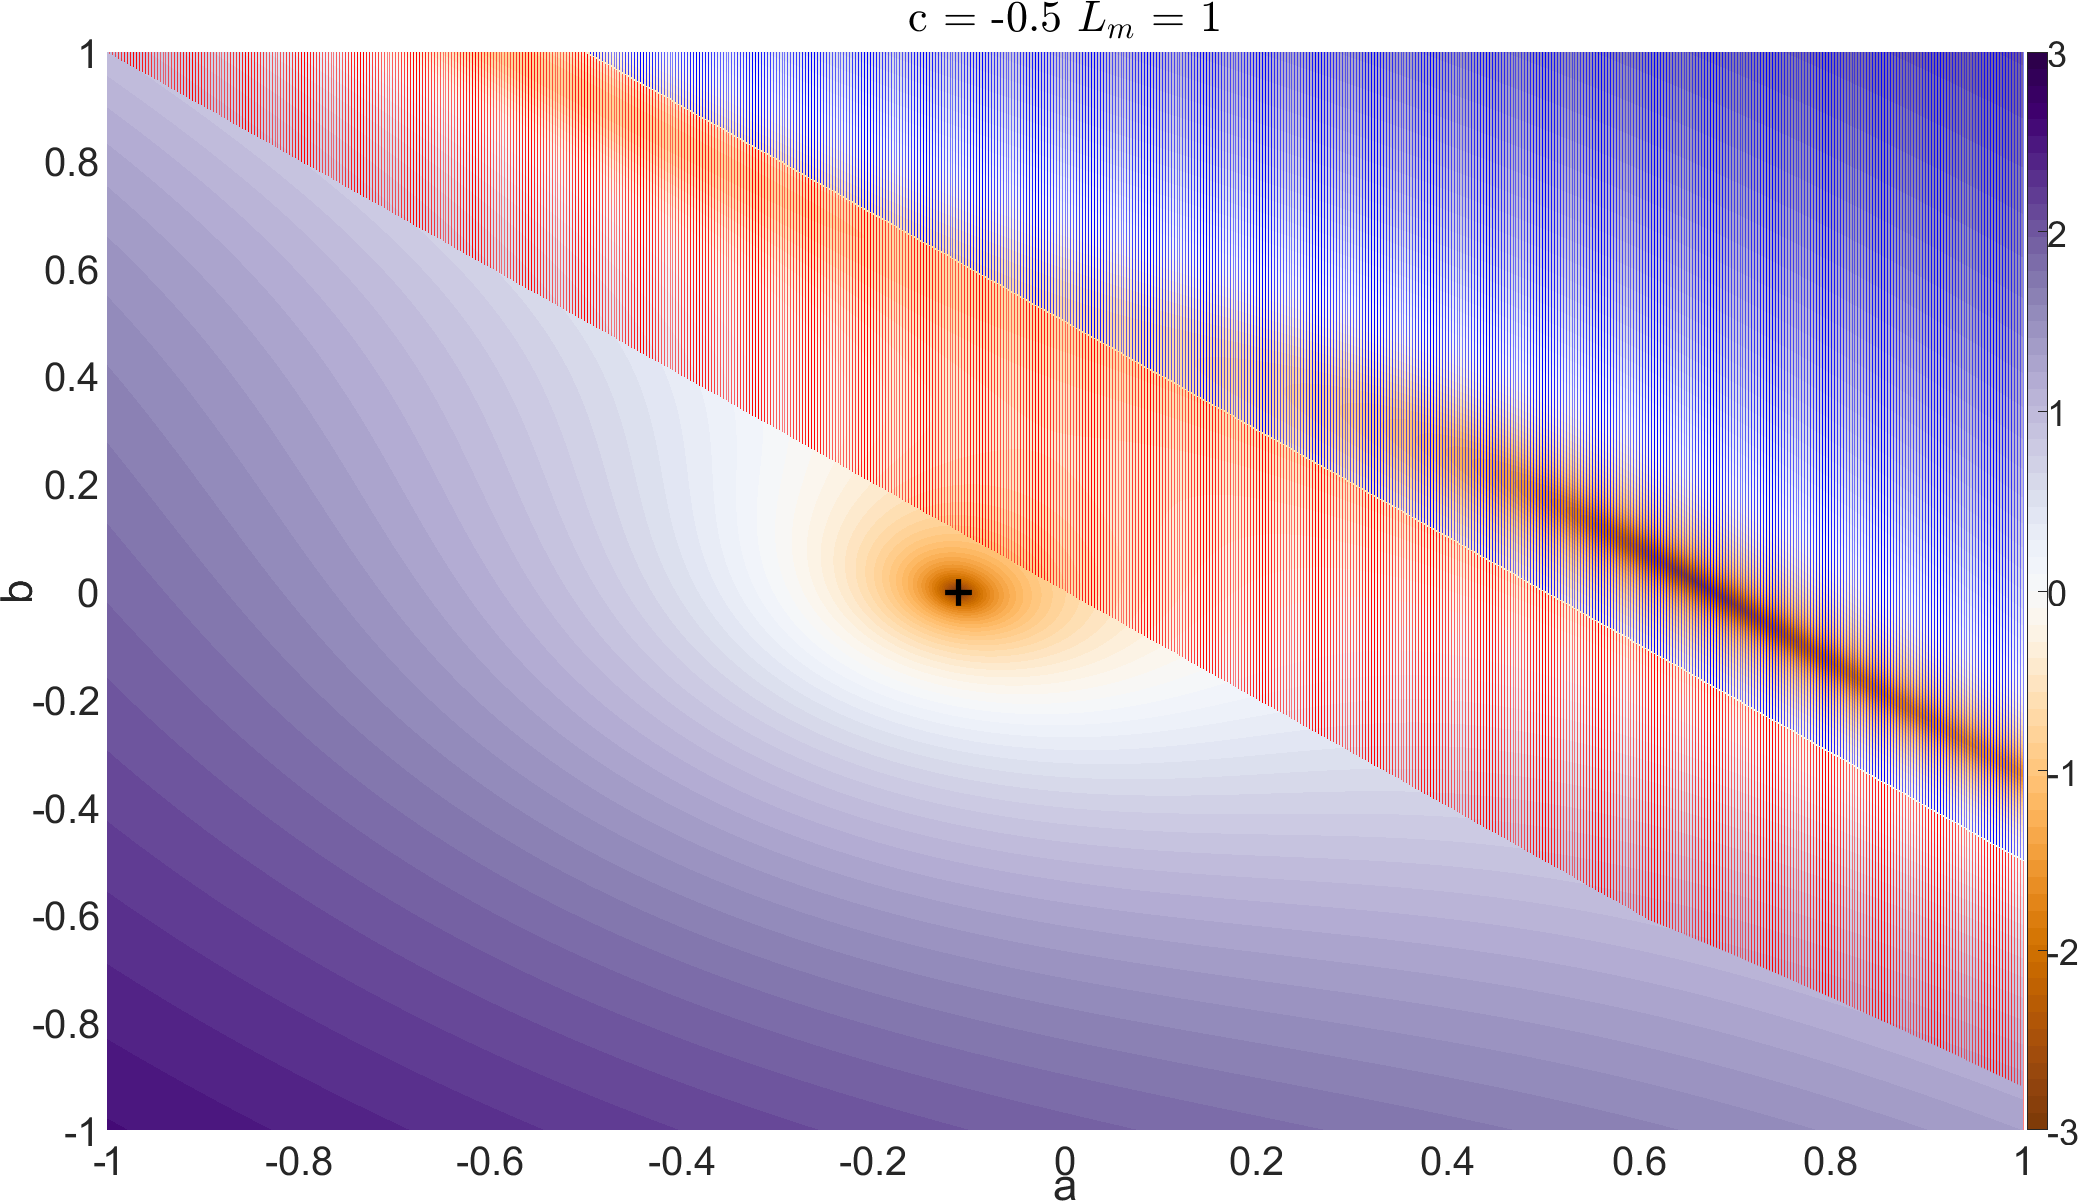
\includegraphics[width = \textwidth]{leastsquaresab.png}
%		\caption{$\log_{10}S(a,b)$}\label{fig:Sab}
%\end{figure}
%\begin{figure}[htbp]
%		\centering 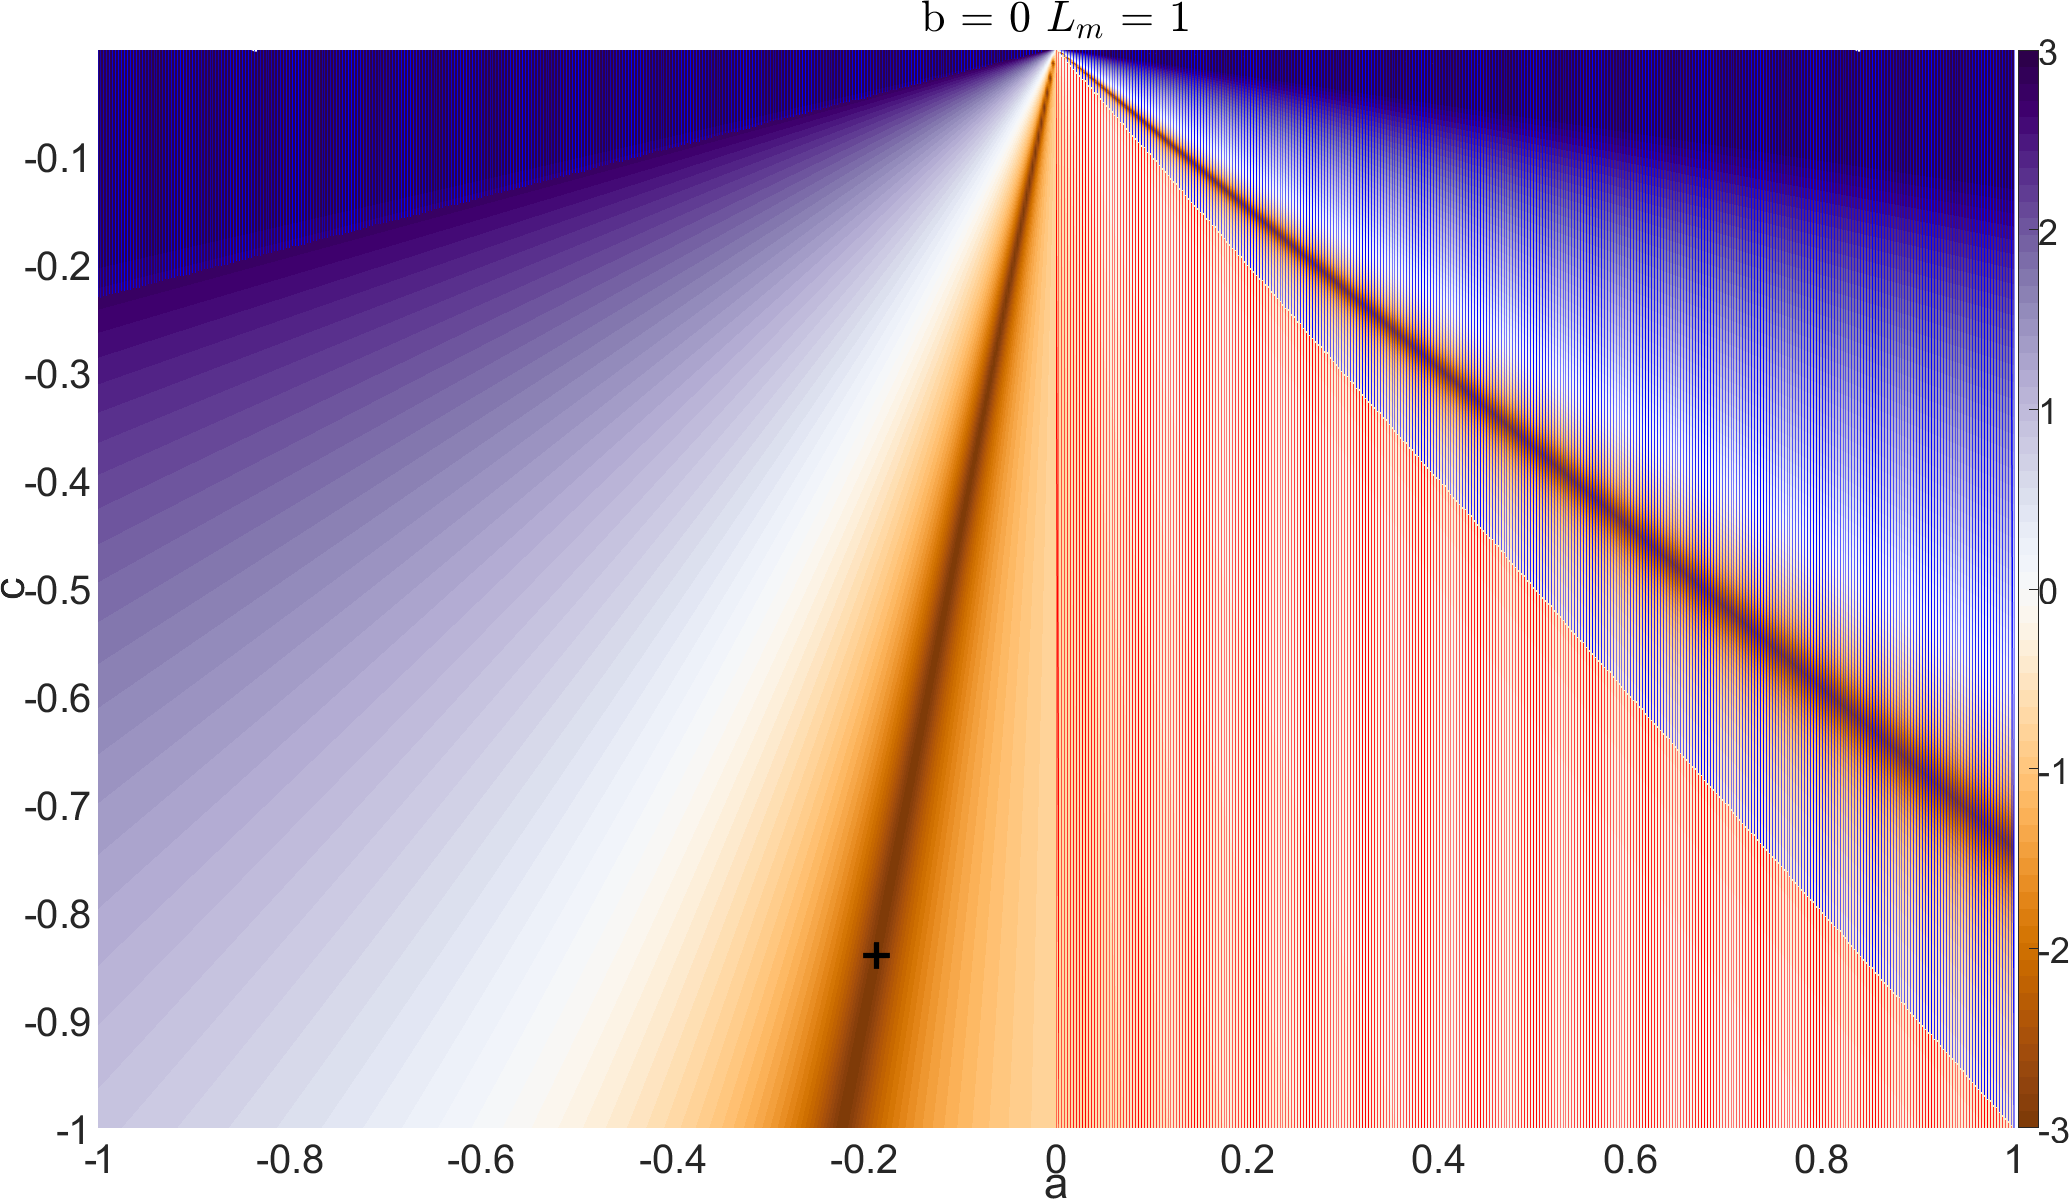
\includegraphics[width = \textwidth]{leastsquaresac.png}
%		\caption{$\log_{10}S(a,c)$}\label{fig:Sac}
%\end{figure}
%\begin{figure}[htbp]
%		\centering 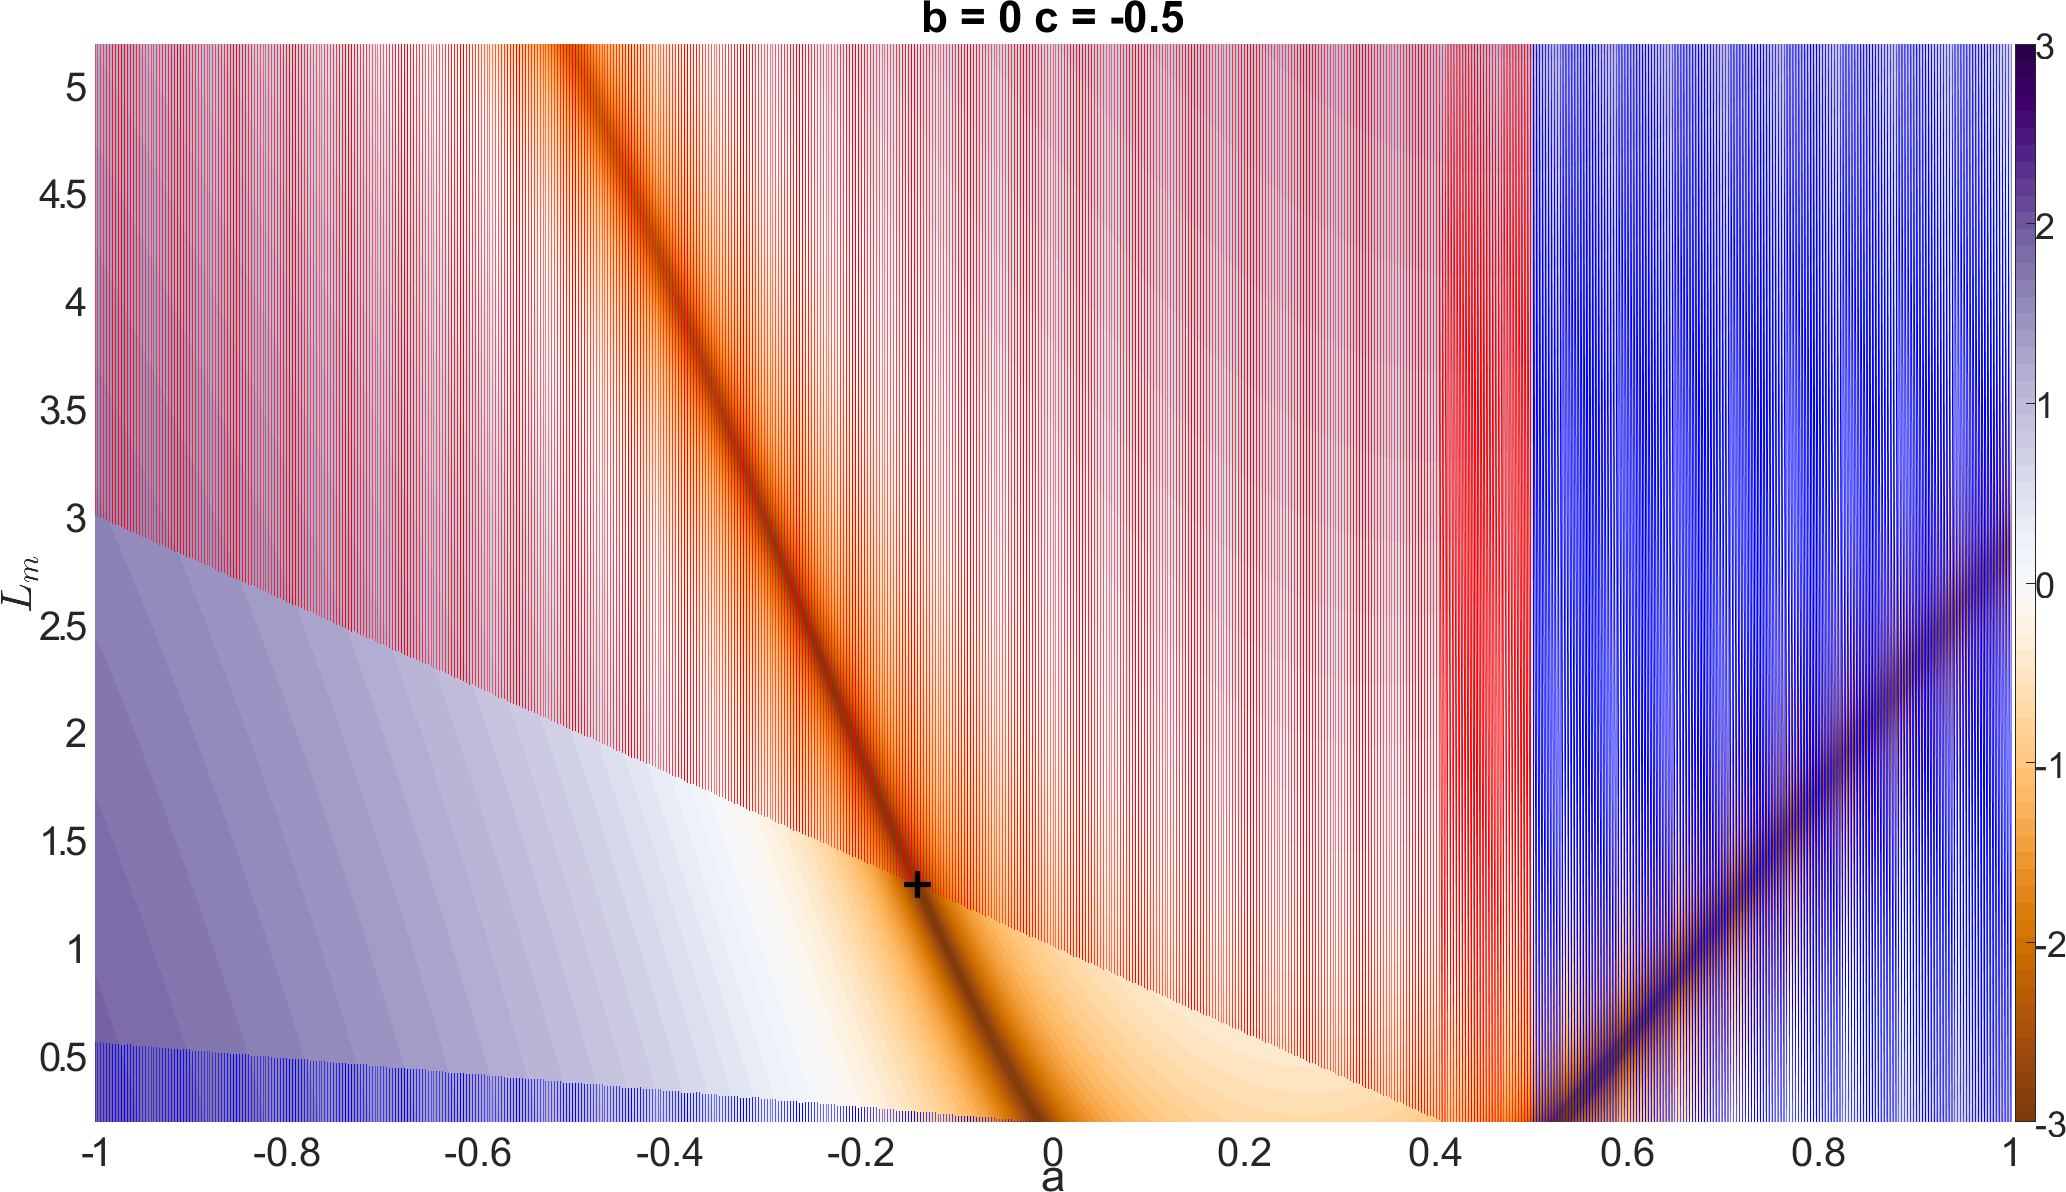
\includegraphics[width = \textwidth]{leastsquaresad.png}
%		\caption{$\log_{10}S(a,d)$}\label{fig:SaLm}
%\end{figure}
%\begin{figure}[htbp]
%		\centering 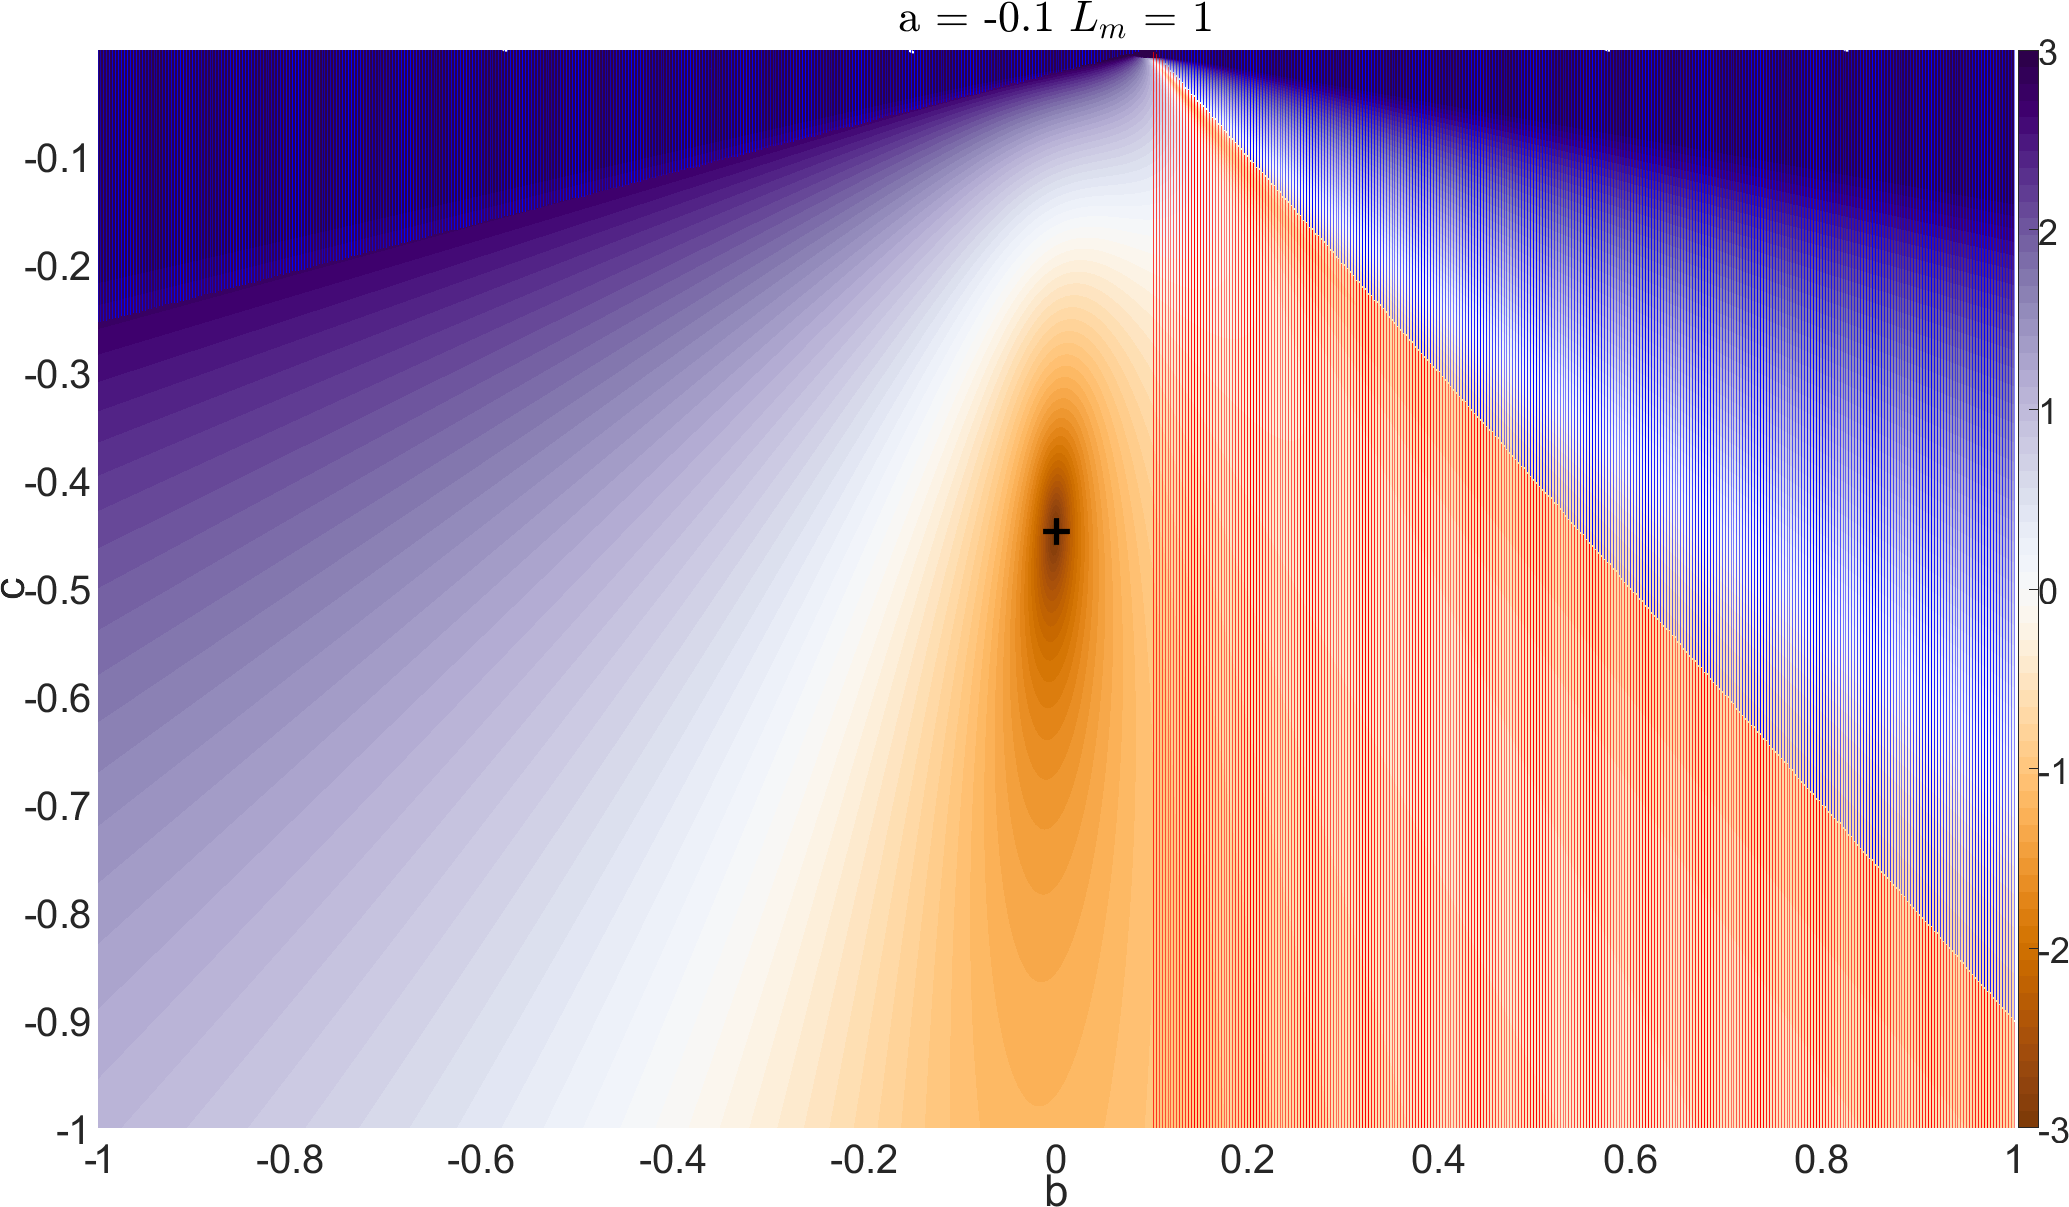
\includegraphics[width = \textwidth]{leastsquaresbc.png}
%		\caption{$\log_{10}S(b,c)$}\label{fig:Sbc}
%\end{figure}
%\begin{figure}[htbp]
%		\centering 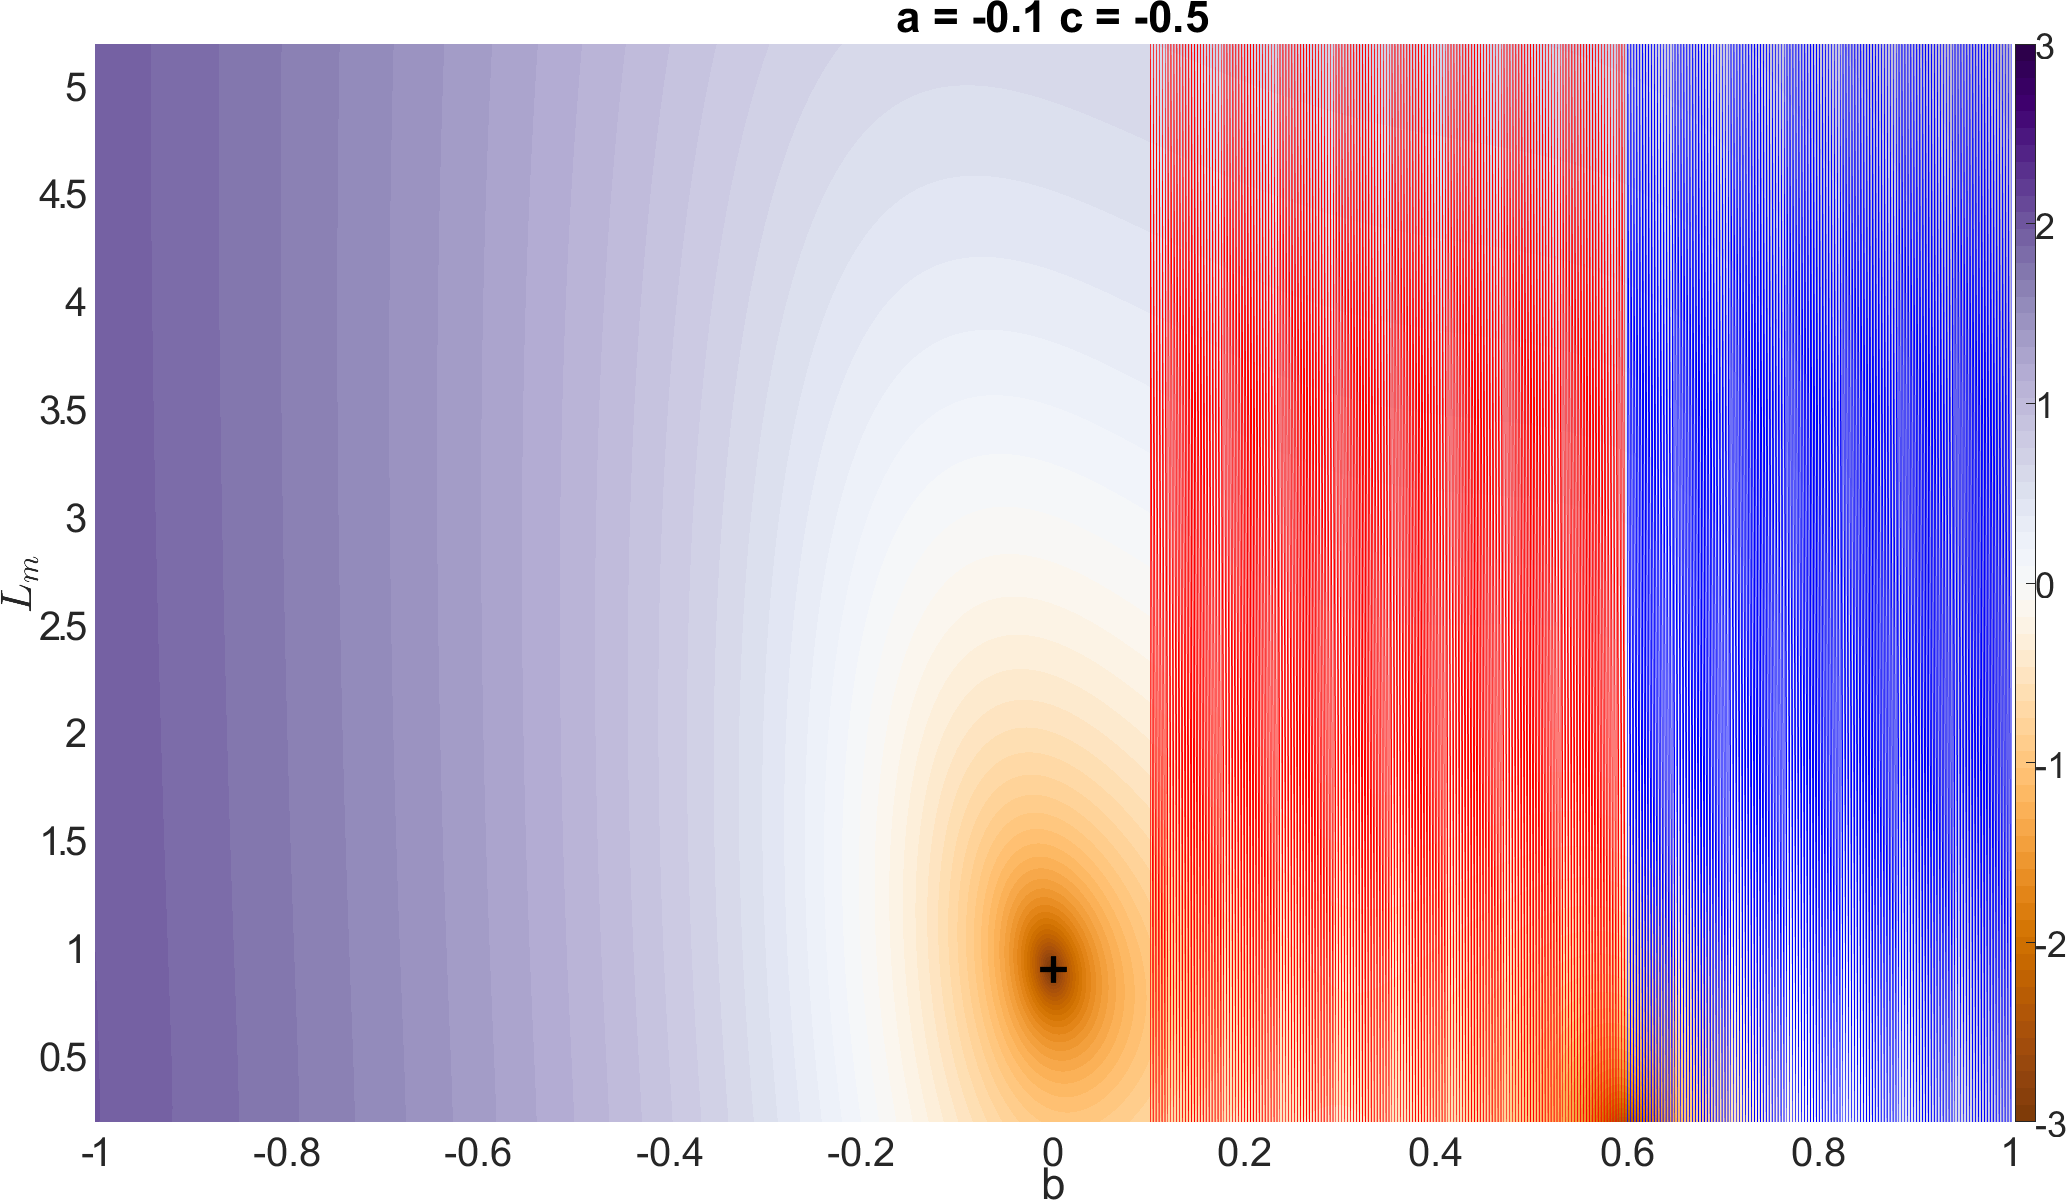
\includegraphics[width = \textwidth]{leastsquaresbd.png}
%		\caption{$\log_{10}S(b,d)$}\label{fig:SbLm}
%\end{figure}
%\begin{figure}[htbp]
%		\centering 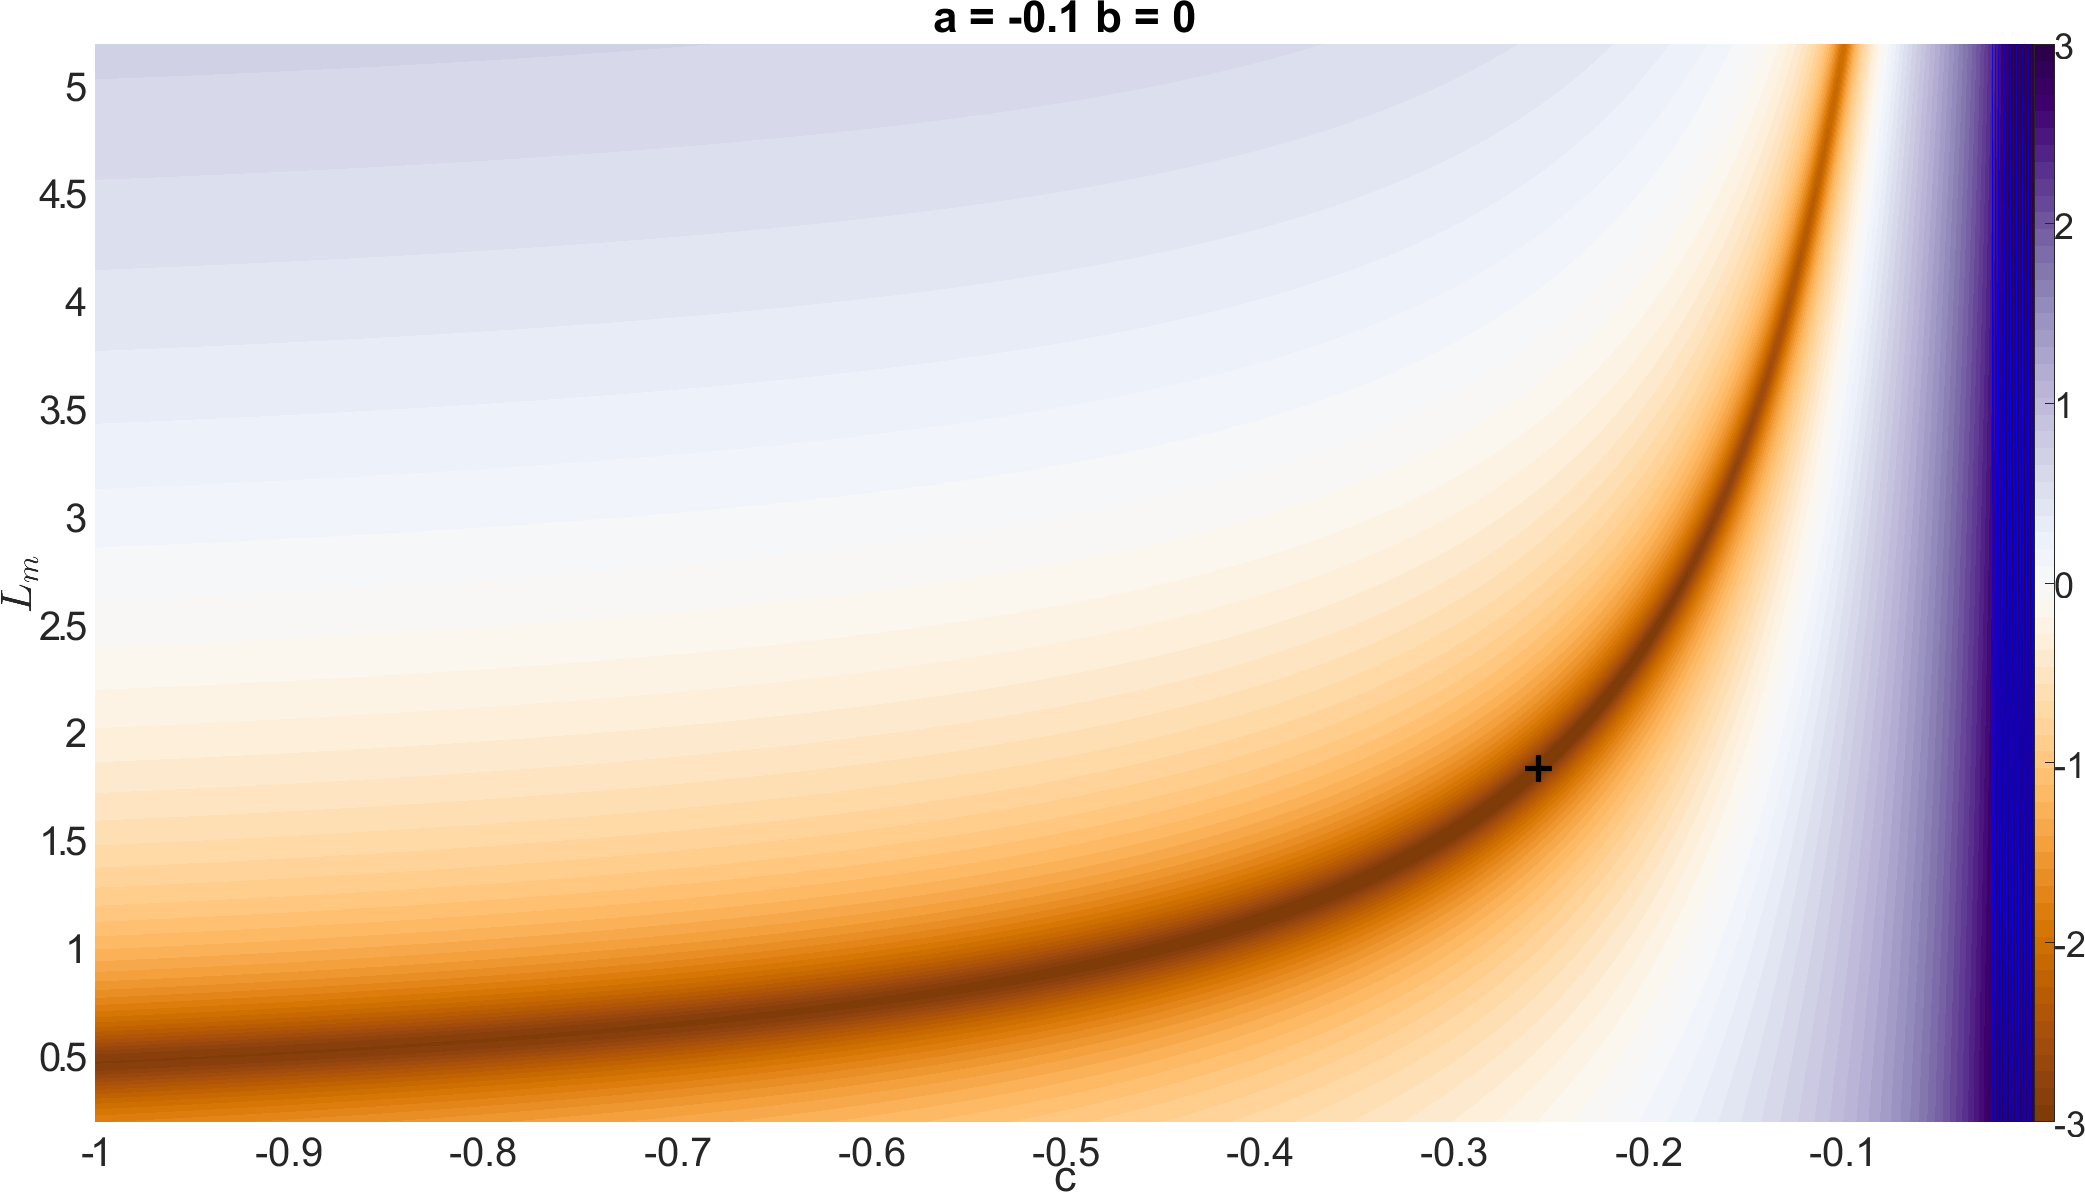
\includegraphics[width = \textwidth]{leastsquarescd.png}
%		\caption{$\log_{10}S(c,d)$}\label{fig:ScLm}
%\end{figure}

\section{Digital Image Correlation}
\label{sec:DIC}
Digital Image Correlation (DIC) is a technique \cite{sutton2009image} to obtain deformation maps from images. We use second-order shape functions \cite{lu2000deformation} to handle large nonlinear deformations. To attain sub-pixel accuracy we interpolate our images with B-splines \cite{thevenaz2000interpolation, unser1999splines}. To obtain the deformations we optimize a Correlation Coefficient, the ZNSSD \cite{sutton2009image}. We solve this nonlinear least-squares problem  by (1) providing an initial guess and (2) solving an iterative scheme. As an initial guess we perform Template Matching \cite{lewis1995industrial,opencv_library} on a limited set of points to obtain rigid deformations with pixel accuracy. After applying DIC to obtain sub-pixel deformations, we use reliability guided DIC \cite{pan2012incremental} with a propagation function \cite{zhou2012propagation} to determine the initial guesses. As iterative scheme we use the LM algorithm. 


\begin{table}[htbp]
\caption{Digital Image Correlation parameters.}
\label{tab:esterrmagn}
\centering
\begin{tabular}{ll}
Noise & \\
Subset Size & \\
Grid Size 	& 5 \\
Measurements Points & \\
Total Number of Images & \\
Number of Averaged Images & \\
Displacements & \\
\qquad Spatial Resolution & x pixels, x mm \\
\qquad Resolution & 0.0105 pixels (x mm) \\
Index of Refraction & \\
\qquad Smoothing Method & \\
\qquad Resolution & x \\
\end{tabular}
\end{table}

Table \ref{tab:esterrmagn} shows the typical DIC parameters used in our experiments. Additionally, the accuracy of the obtained displacements is given.

For practical considerations for DIC we refer to \cite{sutton2009image}, in particular Chapter 10. What was most important for our application was ensuring that the histogram of gray values, from a typical measurement, showed no under- or oversaturation and filled the range of gray values. The under- or oversaturation was solved by changing the intensity of the (uniform) light source. Filling the entire range of gray values was ensured by using a high quality random dot pattern: No sharp edges from black to white, but gradual (gray) changes and having a high enough dot density to ensure a subset has enough information to accurately determine displacements. % Image Averaging $>$ Thermal Noise $>$ Static images

\section{Inverse Model}
\label{sec:invmod}
Looking at our forward model (\ref{eq:ForwardModel}), we know
\begin{enumerate}
	\item $\underline{\alpha}$, the parameters of our experimental setup (after calibration), 
	\item $\underline{x}$, the coordinates on our image sensor, 
	\item $\underline{\Delta x}$, the measured displacement (after DIC), 
	\item $n_0$, the index of refraction of the reference state.
\end{enumerate}
The unknown is the index of refraction field $n$. Unlike the simple model, we cannot invert the forward model to obtain an expression for the index of refraction $n$. We treat the problem of finding $n$ as an optimization problem:
\begin{equation}
\label{eq:nmin} 
	\min_{n_i} (X(n_i, \underline{\alpha}, \underline{x}_i+\underline{\Delta x}_i) - X(n_0, \underline{\alpha}, \underline{x}_i))^2, 
\end{equation}
with constraints $1.333 \leq n_i \leq 1.4$. For each measurement $\underline{\Delta x}_i$ we solve (\ref{eq:nmin}) with the LM algorithm to find $n_i$. In our experiments, (\ref{eq:nmin}) has one minimum in the range $1.333 \leq n_i \leq 1.4$. Picking an initial condition in this range ensures LM finds this minimum.

Since we are working with liquids we use the Lorentz-Lorenz equation to relate the index of refraction $n$ to the density $\rho$ \cite{lorentz1916theory, tan2015dependence},
\begin{equation}
 	\frac{n^2-1}{n^2+2} \frac{1}{\rho} = \mbox{ constant}.
\end{equation}
We use our calibration measurement to determine the constant: $\rho=1$ for $n=1.333$.

\section{Results}
\label{sec:res}
In this section we show three applications of the new method: (1) A static two-layer fluid with large nonlinear deformations, (2) A static stratified fluid and (3) a dynamic fluid/flow? with wave attractor.

In the first application, Figure \ref{fig:0side}, we measured the background density of a two-layer fluid system. We filled the bottom half of a tank with Wadden Sea water (with an index of refraction of 1.338)\footnote{Measured by a refractometer: The Atago Urine Specific Gravity Refractometer with a refractive index range of 1.333-1.356 and a resolution of 0.0005.} and the upper half of the tank with tap water (with an index of refraction of 1.333). We kept the interface between the two layers sharp by filling the upper half of the tank through a sponge. The observed deformations of the dot pattern through this interface are large. Through the use of the second-order shape functions in the DIC procedure, we can still determine these deformations. Figure \ref{fig:ndeformed0side} shows the index of refraction field $n$. The expected theoretical density profile is an error function. We see this in Figure \ref{fig:ndeformed0side}.

\begin{figure}[htbp]
\begin{subfigure}{.5\linewidth}
%		\centering \includegraphics[width = \textwidth]{}
		\subcaption{Reference Image: Filled with air}\label{fig:air0side}
\end{subfigure}%
\begin{subfigure}{.5\linewidth}
%	\centering \includegraphics[width = \textwidth]{}
	\subcaption{Calibration Image Image: Filled with water with known $n$}\label{fig:fresh0side}
\end{subfigure}\\
\begin{subfigure}{.5\linewidth}
%		\centering \includegraphics[width = \textwidth]{}
		\subcaption{Deformed Image: Filled with salt water with unknown $n$-field }\label{fig:twolayer0side}
\end{subfigure}%
\begin{subfigure}{.5\linewidth}
%	\centering \includegraphics[width = \textwidth]{}
	\subcaption{Index of Refraction $n$ for Calibration Image}\label{fig:ncalibration0side}
\end{subfigure}\\
\begin{subfigure}{.5\linewidth}
%		\centering \includegraphics[width = \textwidth]{}
		\subcaption{$\Delta x$ from DIC}\label{fig:dx0side}
\end{subfigure}%
\begin{subfigure}{.5\linewidth}
%	\centering \includegraphics[width = \textwidth]{}
		\subcaption{$\Delta y$ from DIC}\label{fig:dy0side}
\end{subfigure}\\
\begin{subfigure}{.5\linewidth}
%		\centering \includegraphics[width = \textwidth]{}
		\subcaption{Index of Refraction $n$ for Deformed Image}\label{fig:ndeformed0side}
\end{subfigure}%
\begin{subfigure}{.5\linewidth}
%	\centering \includegraphics[width = \textwidth]{}
		\subcaption{Correlation Coefficient from DIC}\label{fig:C0side}
\end{subfigure} \\
\begin{subfigure}{.5\linewidth}
%	\centering \includegraphics[width = \textwidth]{}
		\subcaption{$n$ profiles for Calibration and Deformed Images}\label{fig:nprofiles0side}
\end{subfigure}
\caption{The procedure for obtaining the index of refraction field $n$. We obtain three images: one Reference Image (\ref{fig:air0side}) filled with air, one Calibration Image (\ref{fig:fresh0side}) filled with water without salts and one Deformed Image (\ref{fig:twolayer0side}) filled with water with an unknown $n$-field. Applying DIC between the Reference Image and the Correlation image, we find the displacements $D=(\Delta x, \Delta y)$. Using these displacements $D$ in (\ref{eq:calmin}), we obtain the parameters $\underline{\alpha}$. After calibration, the resulting $n$-field is uniform (\ref{fig:ncalibration0side}). Applying DIC between the Reference Image and the Deformed Image, we find the displacements $\Delta x$ (\ref{fig:dx0side}) and $\Delta y$ (\ref{fig:dy0side}) with corresponding Correlation Coefficient (\ref{fig:C0side}).  Using these displacements in (\ref{eq:nmin}), we obtain the unknown index of refraction field $n$ (\ref{fig:ndeformed0side}). Horizontally averaging the index of refraction fields $n$ yields the profiles in \ref{fig:nprofiles0side}.}
\label{fig:0side}
\end{figure}

\begin{table}[htbp]
\caption{Angles $\beta$ of internal wave beams as a function of the forcing frequency $\omega$. These were determined by a Synthetic Schlieren setup.}
\label{tab:SSintwav}
\centering
\begin{tabular}{llllll}
$\omega$ & 1 & 1 & 1 & 1 & 1  \\
$\beta$  & 1 & 1 & 1 & 1 & 1
\end{tabular}
\end{table}

In the second application, Figure \ref{fig:0side}, we measured the background density of a continuously stratified fluid. We filled a tank through the double bucket method. After taking a Reference Image, a Calibration Image and a Deformed Image, we repositioned the camera for a Synthetic Schlieren measurement. After oscillating the tank, we measured the angles of the internal waves propagating in the fluid. Table \ref{tab:SSintwav} shows the forcing frequencies $\omega$ and angles $\beta$. Through
\begin{equation}
	N = \omega \cos \beta
\end{equation}
we determined the buoyancy frequency $N$. Through
\begin{equation}
	N^2 = - \frac{g}{\rho_0}\frac{d \rho_0}{d z}
\end{equation}
we determined the buoyancy frequency $N$, obtained from our new method. 

\begin{figure}[htbp]
\begin{subfigure}{.5\linewidth}
%		\centering \includegraphics[width = \textwidth]{}
		\subcaption{Deformed Image: Filled with salt water with unknown $n$-field }\label{fig:strat0side}
\end{subfigure}%
\begin{subfigure}{.5\linewidth}
%	\centering \includegraphics[width = \textwidth]{}
		\subcaption{Correlation Coefficient from DIC}\label{fig:stratC0side}
\end{subfigure} \\
\begin{subfigure}{.5\linewidth}
%		\centering \includegraphics[width = \textwidth]{}
		\subcaption{$\Delta x$ from DIC}\label{fig:stratdx0side}
\end{subfigure}%
\begin{subfigure}{.5\linewidth}
%	\centering \includegraphics[width = \textwidth]{}
		\subcaption{$\Delta y$ from DIC}\label{fig:stratdy0side}
\end{subfigure}\\
\begin{subfigure}{.5\linewidth}
%		\centering \includegraphics[width = \textwidth]{}
		\subcaption{Index of Refraction $n$ for Deformed Image}\label{fig:stratndeformed0side}
\end{subfigure}%
\begin{subfigure}{.5\linewidth}
%		\centering \includegraphics[width = \textwidth]{}
		\subcaption{Background Density $\rho_0$ for Deformed Image}\label{fig:stratrho0deformed0side}
\end{subfigure} 
\caption{Determining the background density for a continuously stratified fluid. After taking three images, with the Deformed Image \ref{fig:strat0side}, we obtain the displacements $\Delta x$ in Figure \ref{fig:stratdx0side} and $\Delta y$ in Figure \ref{fig:stratdy0side} from DIC. After calibration we obtain the index of refraction field $n$ in Figure \ref{fig:stratndeformed0side}. Using the Lorentz-Lorenz relation we obtain the density profile \ref{fig:stratrho0deformed0side} with buoyancy frequency $N$ of NUMBER. }
\label{figs:strat0side}
\end{figure}

In the third application, we measured the density field of a wave attractor \cite{maas1997observation}. Figure \ref{figs:WA0side} shows the measured density fields over one period of a (1,1) Wave Attractor. 
\begin{figure}[htbp]
\begin{subfigure}{.5\linewidth}
%		\centering \includegraphics[width = \textwidth]{}
		\subcaption{0}\label{fig:WA0side}
\end{subfigure}%
\begin{subfigure}{.5\linewidth}
%	\centering \includegraphics[width = \textwidth]{}
		\subcaption{P/6}\label{fig:WA6side}
\end{subfigure} \\
\begin{subfigure}{.5\linewidth}
%		\centering \includegraphics[width = \textwidth]{}
		\subcaption{P/3}\label{fig:WA3side}
\end{subfigure}%
\begin{subfigure}{.5\linewidth}
%	\centering \includegraphics[width = \textwidth]{}
		\subcaption{P/2}\label{fig:WA2side}
\end{subfigure} \\
\begin{subfigure}{.5\linewidth}
%		\centering \includegraphics[width = \textwidth]{}
		\subcaption{2P/3}\label{fig:WA23side}
\end{subfigure}%
\begin{subfigure}{.5\linewidth}
%	\centering \includegraphics[width = \textwidth]{}
		\subcaption{5P/6}\label{fig:WA56side}
\end{subfigure} 
\caption{Density Fields over one period of a Wave Attractor. The forcing frequency was NUMBER. }
\label{figs:WA0side}
\end{figure}

\section{Discussion}
\label{sec:dis}

definition planes -> doesn't have to be parallel. in particular 6th plane can be different, extra parameters to estimate in $\alpha$ (calibration). 
non plane water tank: measure without tank, with tank with air -> (calibration) shape of tank, field $L_t$
-> doesn't even have to be planes

Same experimental equipment as BOS or SS - Can apply this method. All complexity is in the image analysis. 

Need to say something about paraxial approximation

The two novel critical steps are: (1) To view the experimental setup under an angle and (2) To calibrate our model. 

Horizontal viewing $\Rightarrow \Delta x, \theta_x$ large. Use $X \Rightarrow \frac{\partial n}{\partial x} = 0$ in static situation.
\begin{acknowledgements}
If you'd like to thank anyone, place your comments here
\end{acknowledgements}

\section*{Funding}
NWO

\section*{Availability of data and material}

\section*{Code availability}

% Authors must disclose all relationships or interests that 
% could have direct or potential influence or impart bias on 
% the work: 
%
 \section*{Conflict of interest}
 The authors declare that they have no conflict of interest.

\printbibliography[heading=bibintoc]
% BibTeX users please use one of
%\bibliographystyle{spbasic}      % basic style, author-year citations
%\bibliographystyle{spmpsci}      % mathematics and physical sciences
%\bibliographystyle{spphys}       % APS-like style for physics
%\bibliography{}   % name your BibTeX data base

% Non-BibTeX users please use
%\begin{thebibliography}{}
%
% and use \bibitem to create references. Consult the Instructions
% for authors for reference list style.
%
%\bibitem{RefJ}
% Format for Journal Reference
%Author, Article title, Journal, Volume, page numbers (year)
% Format for books
%\bibitem{RefB}
%Author, Book title, page numbers. Publisher, place (year)
% etc
%\end{thebibliography}

\end{document}
% end of file template.tex

